\chapter{体积自锁问题}
本章首先介绍了体积不可压材料的弹性力学问题,及其伽辽金求解过程中存在的体积自锁现象。
针对该问题,介绍了罚函数型和拉格朗日乘子型两类解决方法,并讨论了这两类方法的等价性。同时,阐述了如何衡量体积自锁程度,包括体积约束比和LBB稳定性条件。

\section{体积不可压材料}               
考虑如图\ref{model}所示维度为$n_d$具有边界$\Gamma$的体积不可压材料弹性体$\Omega\in \mathbb R^{n_d}$,其中$\Gamma_t$和$\Gamma_g$分别表示其自然边界和本质边界,
且$\Gamma_t \cup \Gamma_g = \Gamma$, $\Gamma_t \cap \Gamma_g = \varnothing$。该问题相应的强形式为:
\begin{equation}\label{strong_penalty}
    \begin{cases}
        \nabla \cdot \boldsymbol \sigma + \boldsymbol b = \boldsymbol 0 & \mathrm{in} \; \Omega \\
        \boldsymbol \sigma \cdot \boldsymbol n = \boldsymbol t & \mathrm{on} \; \Gamma_t \\
        \boldsymbol u = \boldsymbol g & \mathrm{on} \; \Gamma_g \\
\end{cases}
\end{equation}
其中$\boldsymbol \sigma$为应力张量,对于各向同性线弹性材料,其本构关系表示为:
\begin{equation}\label{stress_penalty}
    \boldsymbol \sigma(\boldsymbol u) = 3\kappa \boldsymbol \varepsilon^v(\boldsymbol u) + 2\mu \boldsymbol \varepsilon^d(\boldsymbol u) 
\end{equation}
式中$\boldsymbol \varepsilon^v$ 和 $\boldsymbol \varepsilon^d$ 为应变张量$\boldsymbol \varepsilon$的体积应变和偏应变部分:
\begin{equation}
    \boldsymbol \varepsilon^v(\boldsymbol u) =\frac{1}{3} \nabla \cdot \boldsymbol u \; \boldsymbol 1, \quad
    \boldsymbol \varepsilon^d(\boldsymbol u) =\frac{1}{2}(\boldsymbol u \nabla + \nabla \boldsymbol u) - \boldsymbol \varepsilon^v, \quad
    \boldsymbol \varepsilon^v : \boldsymbol \varepsilon^d = 0
\end{equation}
其中,$\boldsymbol 1 = \delta_{ij} \boldsymbol e_i \otimes \boldsymbol e_j$是二阶恒等张量。$\kappa$, $\mu$ 分别为体积模量和剪切模量,其与杨氏模量$E$和泊松比$\nu$之间存在如下关系式:
\begin{equation}\label{modulus}
    \kappa = \frac{E}{3(1-2\nu)}, \quad \mu = \frac{E}{2(1+\nu)}
\end{equation}
$\boldsymbol b$为$\Omega$中的体力, $\boldsymbol t$, $\boldsymbol g$ 分别为自然边界$\Gamma_t$和本质边界$\Gamma_g$上的牵引力和位移。

\begin{figure}[!h]
    \centering 
        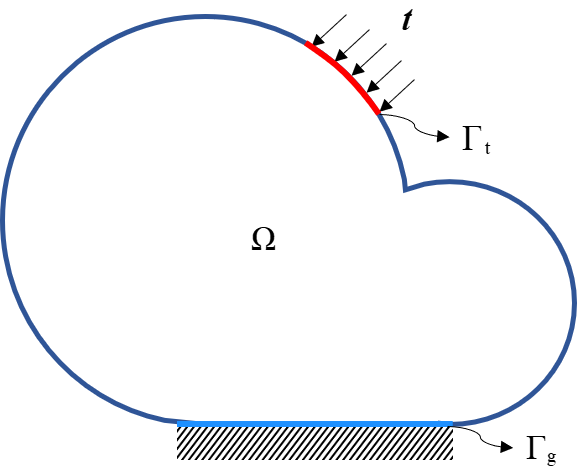
\includegraphics[scale=0.7]{figures/model.png}
        \caption{不可压缩材料弹性体模型}\label{model}
\end{figure}

对于体积不可压缩材料,其泊松比$\nu \rightarrow 0.5$。 在这种情况下,式\eqref{modulus}中体积模量$\kappa \rightarrow \infty$,而剪切模量$\mu$的变化相对较小,从而导致$\kappa\gg\mu$。
根据体积不可压缩材料本构关系\eqref{stress_penalty},当$\kappa \rightarrow \infty$时,体积应变$\boldsymbol \varepsilon^v$被约束,导致体积的变化$\nabla \cdot \boldsymbol u\rightarrow 0$。

采用伽辽金法进行求解时,其相对应的伽辽金弱形式为:
位移$\boldsymbol u \in V$满足
\begin{equation}\label{weak_penalty}
\int_\Omega 2\mu \delta \boldsymbol \varepsilon^d : \boldsymbol \varepsilon^d d\Omega +
\int_\Omega 3\kappa \delta \boldsymbol \varepsilon^v : \boldsymbol \varepsilon^v d\Omega =
\int_{\Gamma_t} \delta \boldsymbol u \cdot \boldsymbol t d\Gamma + \int_\Omega \delta \boldsymbol u \cdot \boldsymbol b d\Omega, \quad
\forall \delta \boldsymbol u \in V
\end{equation}
其中,空间$V=\{\boldsymbol v \in H^1(\Omega)^2\;\vert\;\boldsymbol v = \boldsymbol g, \; \textrm{on} \; \Gamma_g\}$。
$\delta\boldsymbol \varepsilon^v$和$\delta\boldsymbol \varepsilon^d $分别为$\delta \boldsymbol u$表示的体积应变和偏应变的变分。

在传统有限元法中,整个求解域$\Omega$可离散为一组节点$\{\boldsymbol x_I\}_{I=1}^{n_u}$表示\cite{hughes2000},其中$n_u$是位移节点的数量。
位移$\boldsymbol u$及其变分$\delta \boldsymbol u $可通过$\boldsymbol x_I$处的节点系数和形函数进行近似:
\begin{equation}\label{u_h}
    \boldsymbol u_h(\boldsymbol x) = \sum_{I=1}^{n_u} N_I(\boldsymbol x) \boldsymbol u_I, \quad
    \delta \boldsymbol u_h(\boldsymbol x) = \sum_{I=1}^{n_u} N_I(\boldsymbol x) \delta \boldsymbol u_I
\end{equation}
其中$N_I$和$\boldsymbol u_I$分别为节点$x_I$处的形函数和节点系数张量。
\begin{figure}[H]
    \centering 
        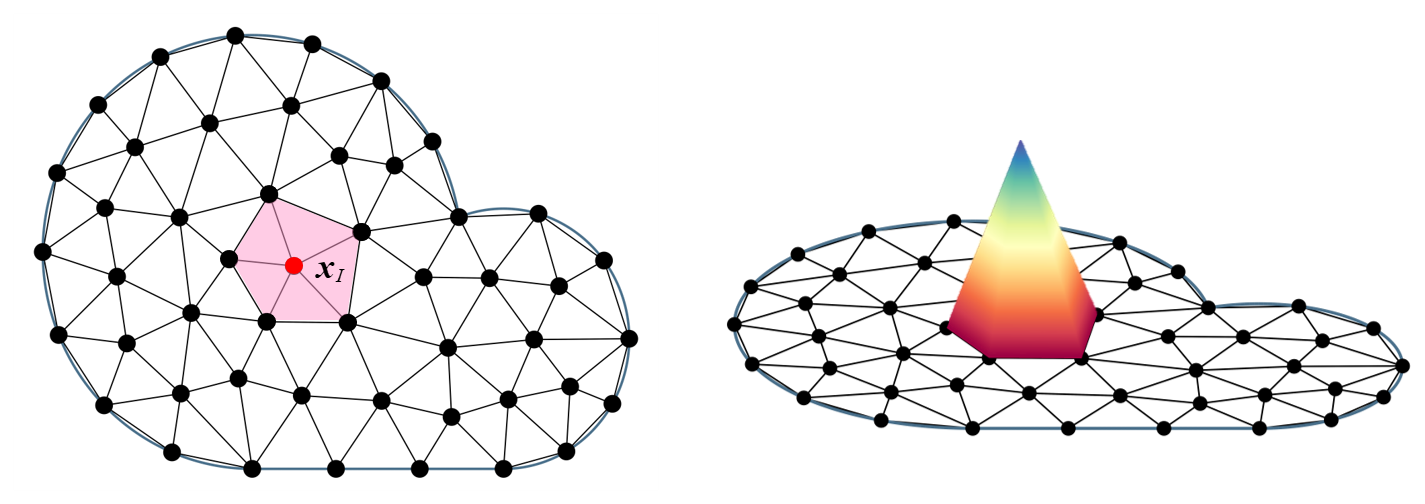
\includegraphics[scale=1.5]{figures/fem.png}
        \caption{有限元离散示意图}\label{fem}
\end{figure}

将式\eqref{u_h}代入到弱形式\eqref{weak_penalty}中可得下列的里兹--伽辽金问题:
近似位移 $\boldsymbol u_h \in V_h$满足
\begin{equation}\label{ritz_penalty}
\int_\Omega 2\mu \delta \boldsymbol \varepsilon^d_h : \boldsymbol \varepsilon^d_h d\Omega +
\int_\Omega 3\kappa \delta \boldsymbol \varepsilon^v_h : \boldsymbol \varepsilon^v_h d\Omega =
\int_{\Gamma_t} \delta \boldsymbol u_h \cdot \boldsymbol t d\Gamma + \int_\Omega \delta \boldsymbol u_h \cdot \boldsymbol b d\Omega, \quad
\forall \delta \boldsymbol u_h \in V_h
\end{equation}
其中近似空间$V_h \subseteq V$,$V_h = \{\boldsymbol v_h \in (\mathrm{span}\{N_I\}_{I=1}^{n_u})^{n_d} \vert \boldsymbol v_h = \boldsymbol g,\; \mathrm{on} \; \Gamma_g\}$。
根据$\delta \boldsymbol u_h$的任意性,等式两边同时消除$\delta \boldsymbol u_I$,上述方程可以简化为如下离散控制方程:
\begin{equation}\label{equilibrium_penalty}
    (\boldsymbol K^d +\boldsymbol K^v) \boldsymbol d^u = \boldsymbol f
\end{equation}
其中,$\boldsymbol d^u$ 是包含 $\boldsymbol u_I$的系数向量,$\boldsymbol K^v$ 为主应力刚度矩阵,$\boldsymbol K^d$为偏应力刚度矩阵,$\boldsymbol f$为力向量,其分量分别为:
\begin{equation}\label{stiffness_vol}
    \boldsymbol K^v_{IJ}=  3\kappa\int_{\Omega} \boldsymbol B^{v\mathrm T}_I \boldsymbol B^v_J d\Omega
\end{equation}
\begin{equation}\label{stiffness_dev}
    \boldsymbol K^d_{IJ}= 2\mu\int_{\Omega} \boldsymbol B^{d\mathrm T}_I \boldsymbol B^d_J d\Omega
\end{equation}
\begin{equation}
    \boldsymbol f_I = \int_{\Gamma_t} N_I \boldsymbol t d\Gamma + \int_{\Omega} N_I \boldsymbol b d\Omega
\end{equation}
式中$\boldsymbol B_I$为形函数梯度矩阵,在二维问题中$\boldsymbol B_I$具有如下表达式:
\begin{equation}\label{strain vector}
    \pmb{B}_I= \left[\begin{matrix}N_{I,x}&0\\0&N_{I,y}\\N_{I,y}&N_{I,x} \end{matrix}\right] 
\end{equation}
\section{免体积自锁方案}
\subsection{罚函数法与缩减积分方案}
由式\eqref{equilibrium_penalty,stiffness_vol}可知,对于体积不可压材料,当外力向量$\boldsymbol f$具有一定的数值时,$\kappa \rightarrow \infty$将导致主应力刚度矩阵$\boldsymbol K^v$中的所有模态也趋向零。
此时,体积刚度矩阵$\boldsymbol K^v$可作为罚函数项将主应力刚度矩阵中所有模态约束住,体积模量$\kappa$为其中的罚因子。
使用传统有限元法进行求解时,由于离散的有限元近似阶次较低,导致过多的位移自由度受到体积约束的限制,位移解将远小于实际情况,即出现体积自锁现象。
% 而体积刚度矩阵的秩$\mathrm{rank}(\boldsymbol K^v)$即为被约束的自由度个数,由式\eqref{stiffness_vol}可知,$\mathrm{rank}(\boldsymbol K^v)$具有如下关系:
% \begin{equation}\label{rank1}
%     \mathit{rank}(\boldsymbol K^v)\le\text{min}(\mathit{rank}( \boldsymbol B^v))
% \end{equation}

引入数值积分实现体积刚度矩阵\eqref{stiffness_vol},有:
\begin{equation}\label{integration}
    \boldsymbol K^v_{IJ} =  3\kappa \sum_{C=1}^{n_e}\sum_{G=1}^{n_g} \boldsymbol B^{vT}_I(\boldsymbol x_G) \boldsymbol B^v_J(\boldsymbol x_G) w_G
\end{equation}
式中,$\boldsymbol x_G$和$w_G$分别为积分点的位置和权重。$n_e$是单元的数量,$n_g$是每个单元中积分点的数量。当引入数值积分后,$\boldsymbol K^v$将要求体积约束在所有数值积分点处满足,$\mathrm{rank}(\boldsymbol k^v)$将受限于数值积分点数量:
\begin{equation}\label{rank}
    \mathrm{rank}(\boldsymbol K^v)\le n_e \times n_g
\end{equation}

FIXME
由式\eqref{rank}可知,减少用于体积刚度矩阵得积分点数量可以减少体积自锁约束。
如图\ref{reduced}所示的经典二维四边形单元(Quad4)缩减积分方案为例,Quad4单元需要采用$2\times2$高斯积分点以保证数值精度,称之为完全积分方案。
为了缓解体积自锁现象,Quad4单元在对主应力刚度矩阵$\boldsymbol K^v$进行数值积分时,采用1点高斯积分作为缩减积分方案。
此时,被约束的自由度个数将被单元数$n_e$限制:
\begin{equation}
    \mathit{rank}(\boldsymbol K^v)\le n_e
\end{equation}

需要指出在有限元离散中,单元数量$n_e$将原小于自由度个数$2n_u$。
如单边单元数为$n$的正方形均布有限元离散,此时的单元数量为$n_e = n^2$,而位移自由度个数为$2n_u = 2(n+1)^2 = 2n^2+2n+1$,$n_e < 2n_u$,
体积自锁现象得以缓解。

\begin{figure}[!h]
    \centering
        \begin{tabular}{c@{\hspace{24pt}}c}
            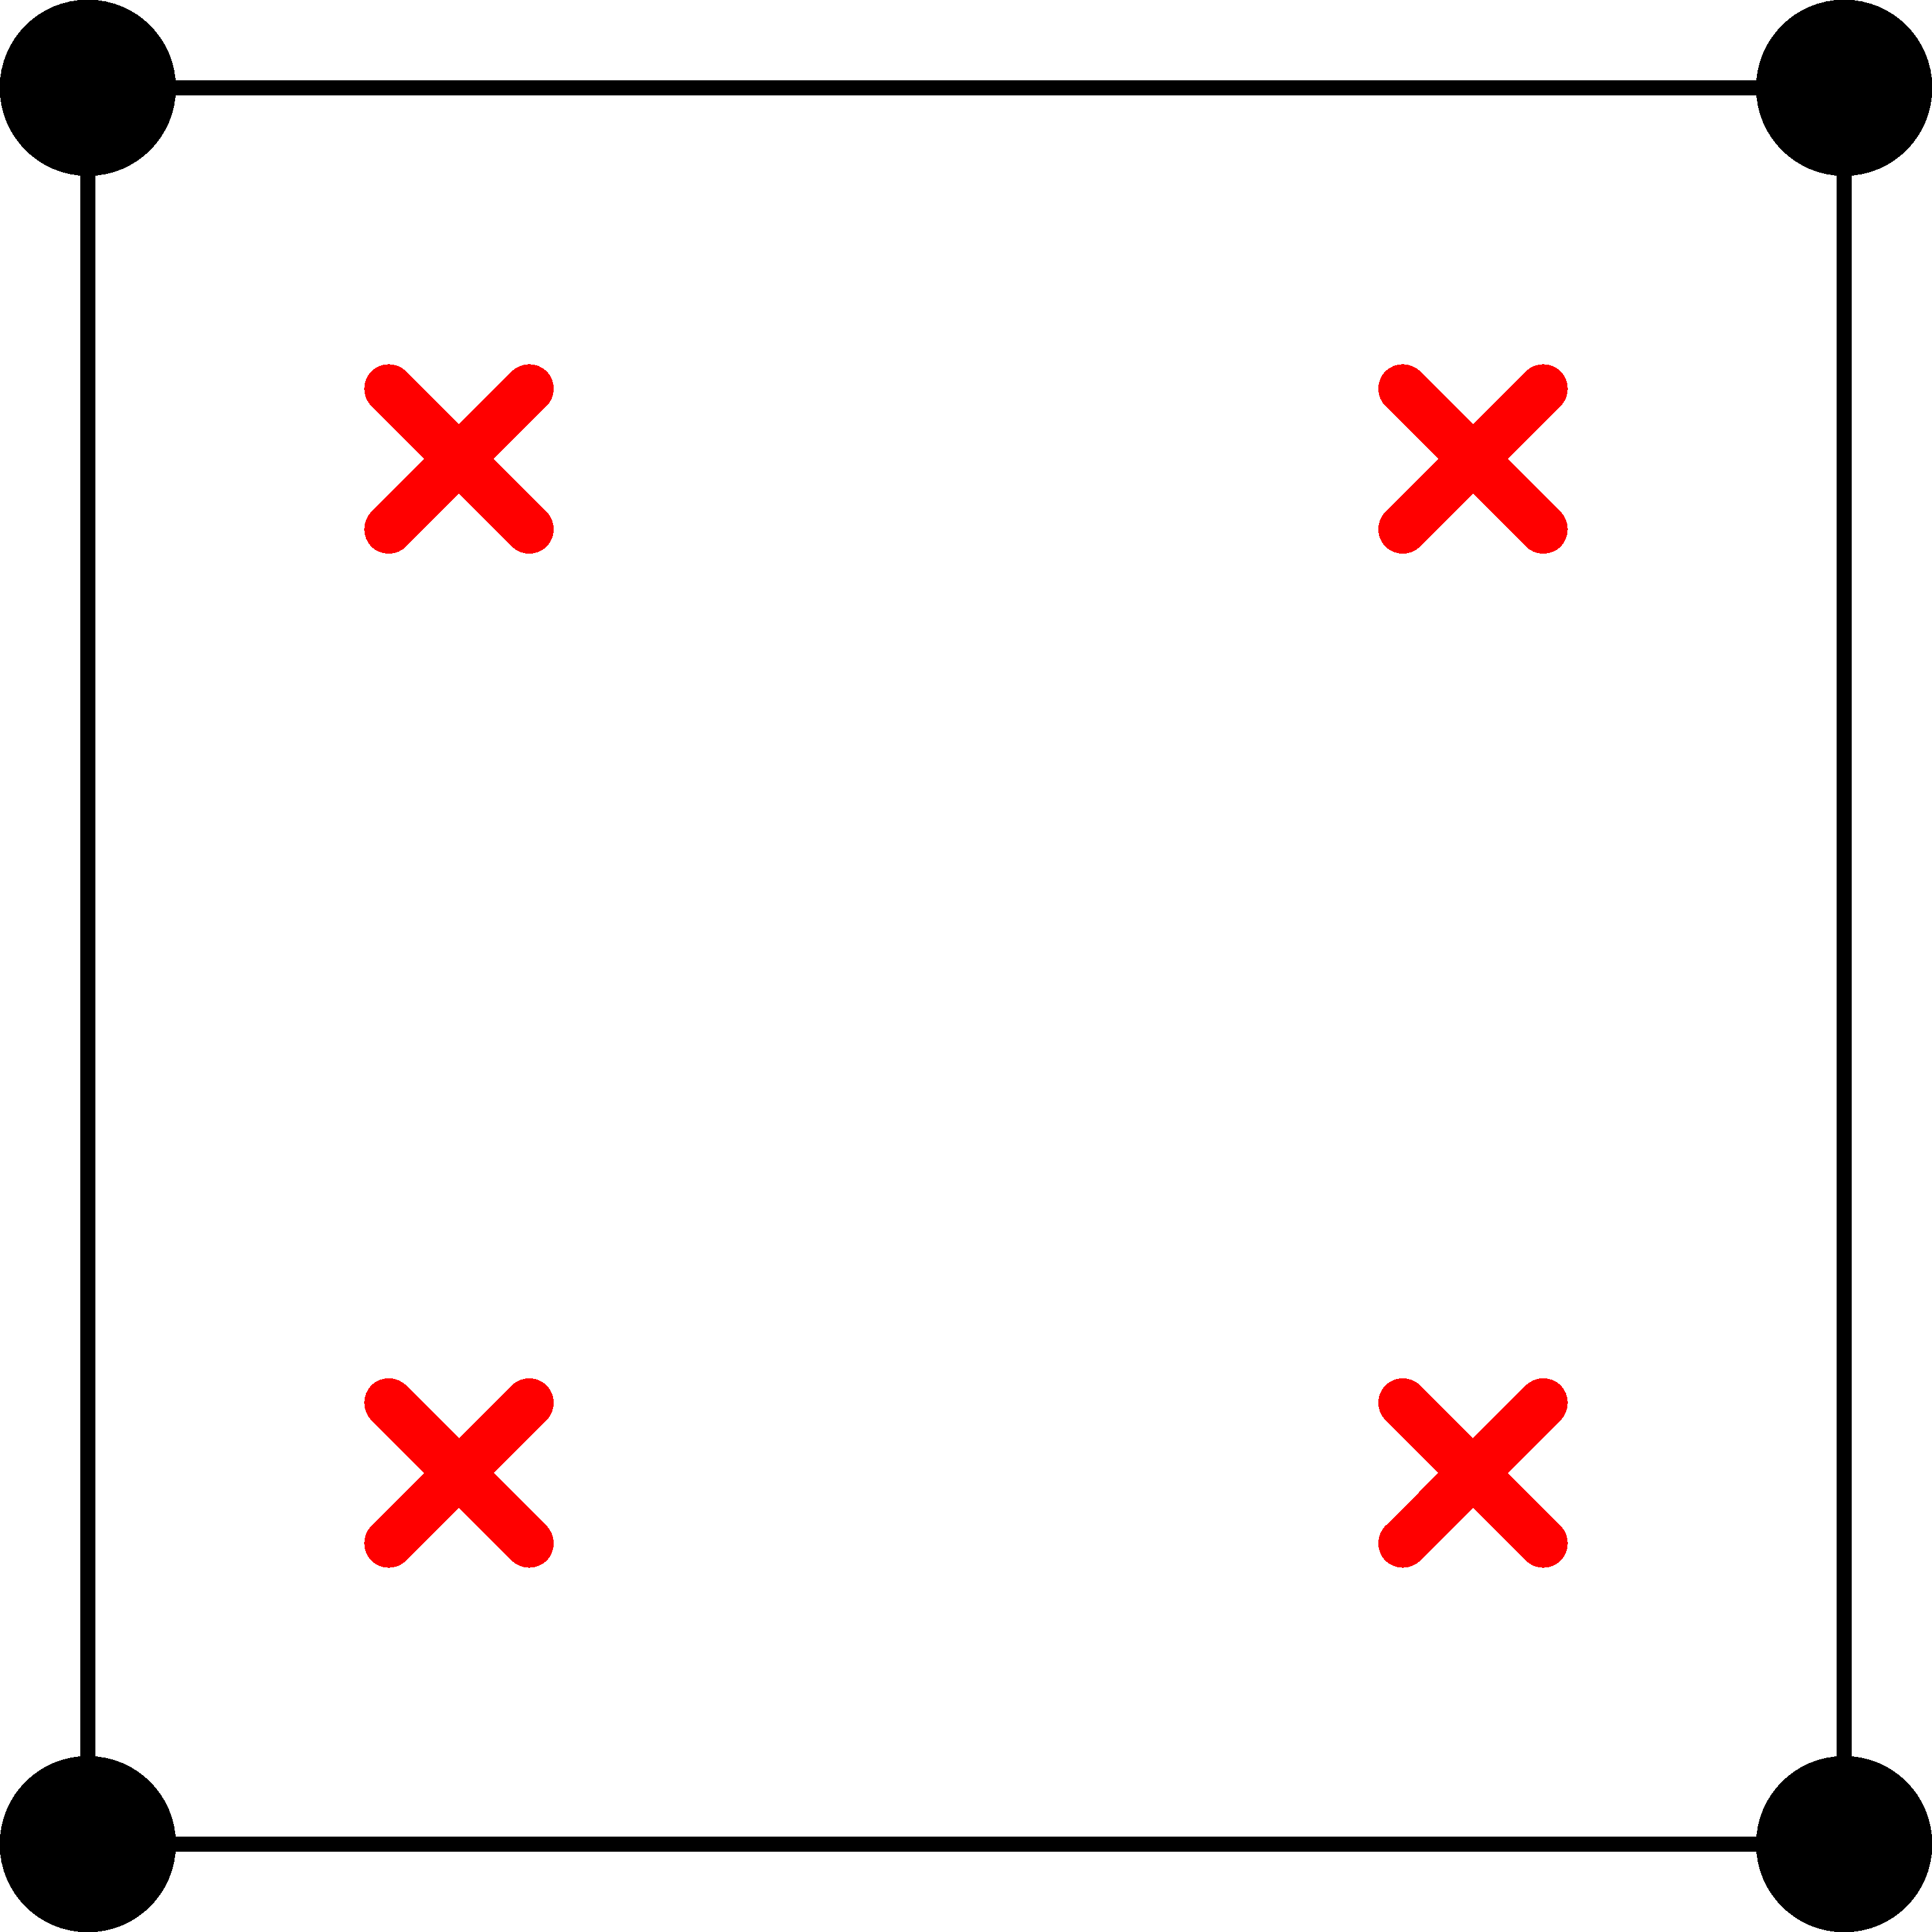
\includegraphics[width=0.3\textwidth]{figures/rd_quad4.png} &
            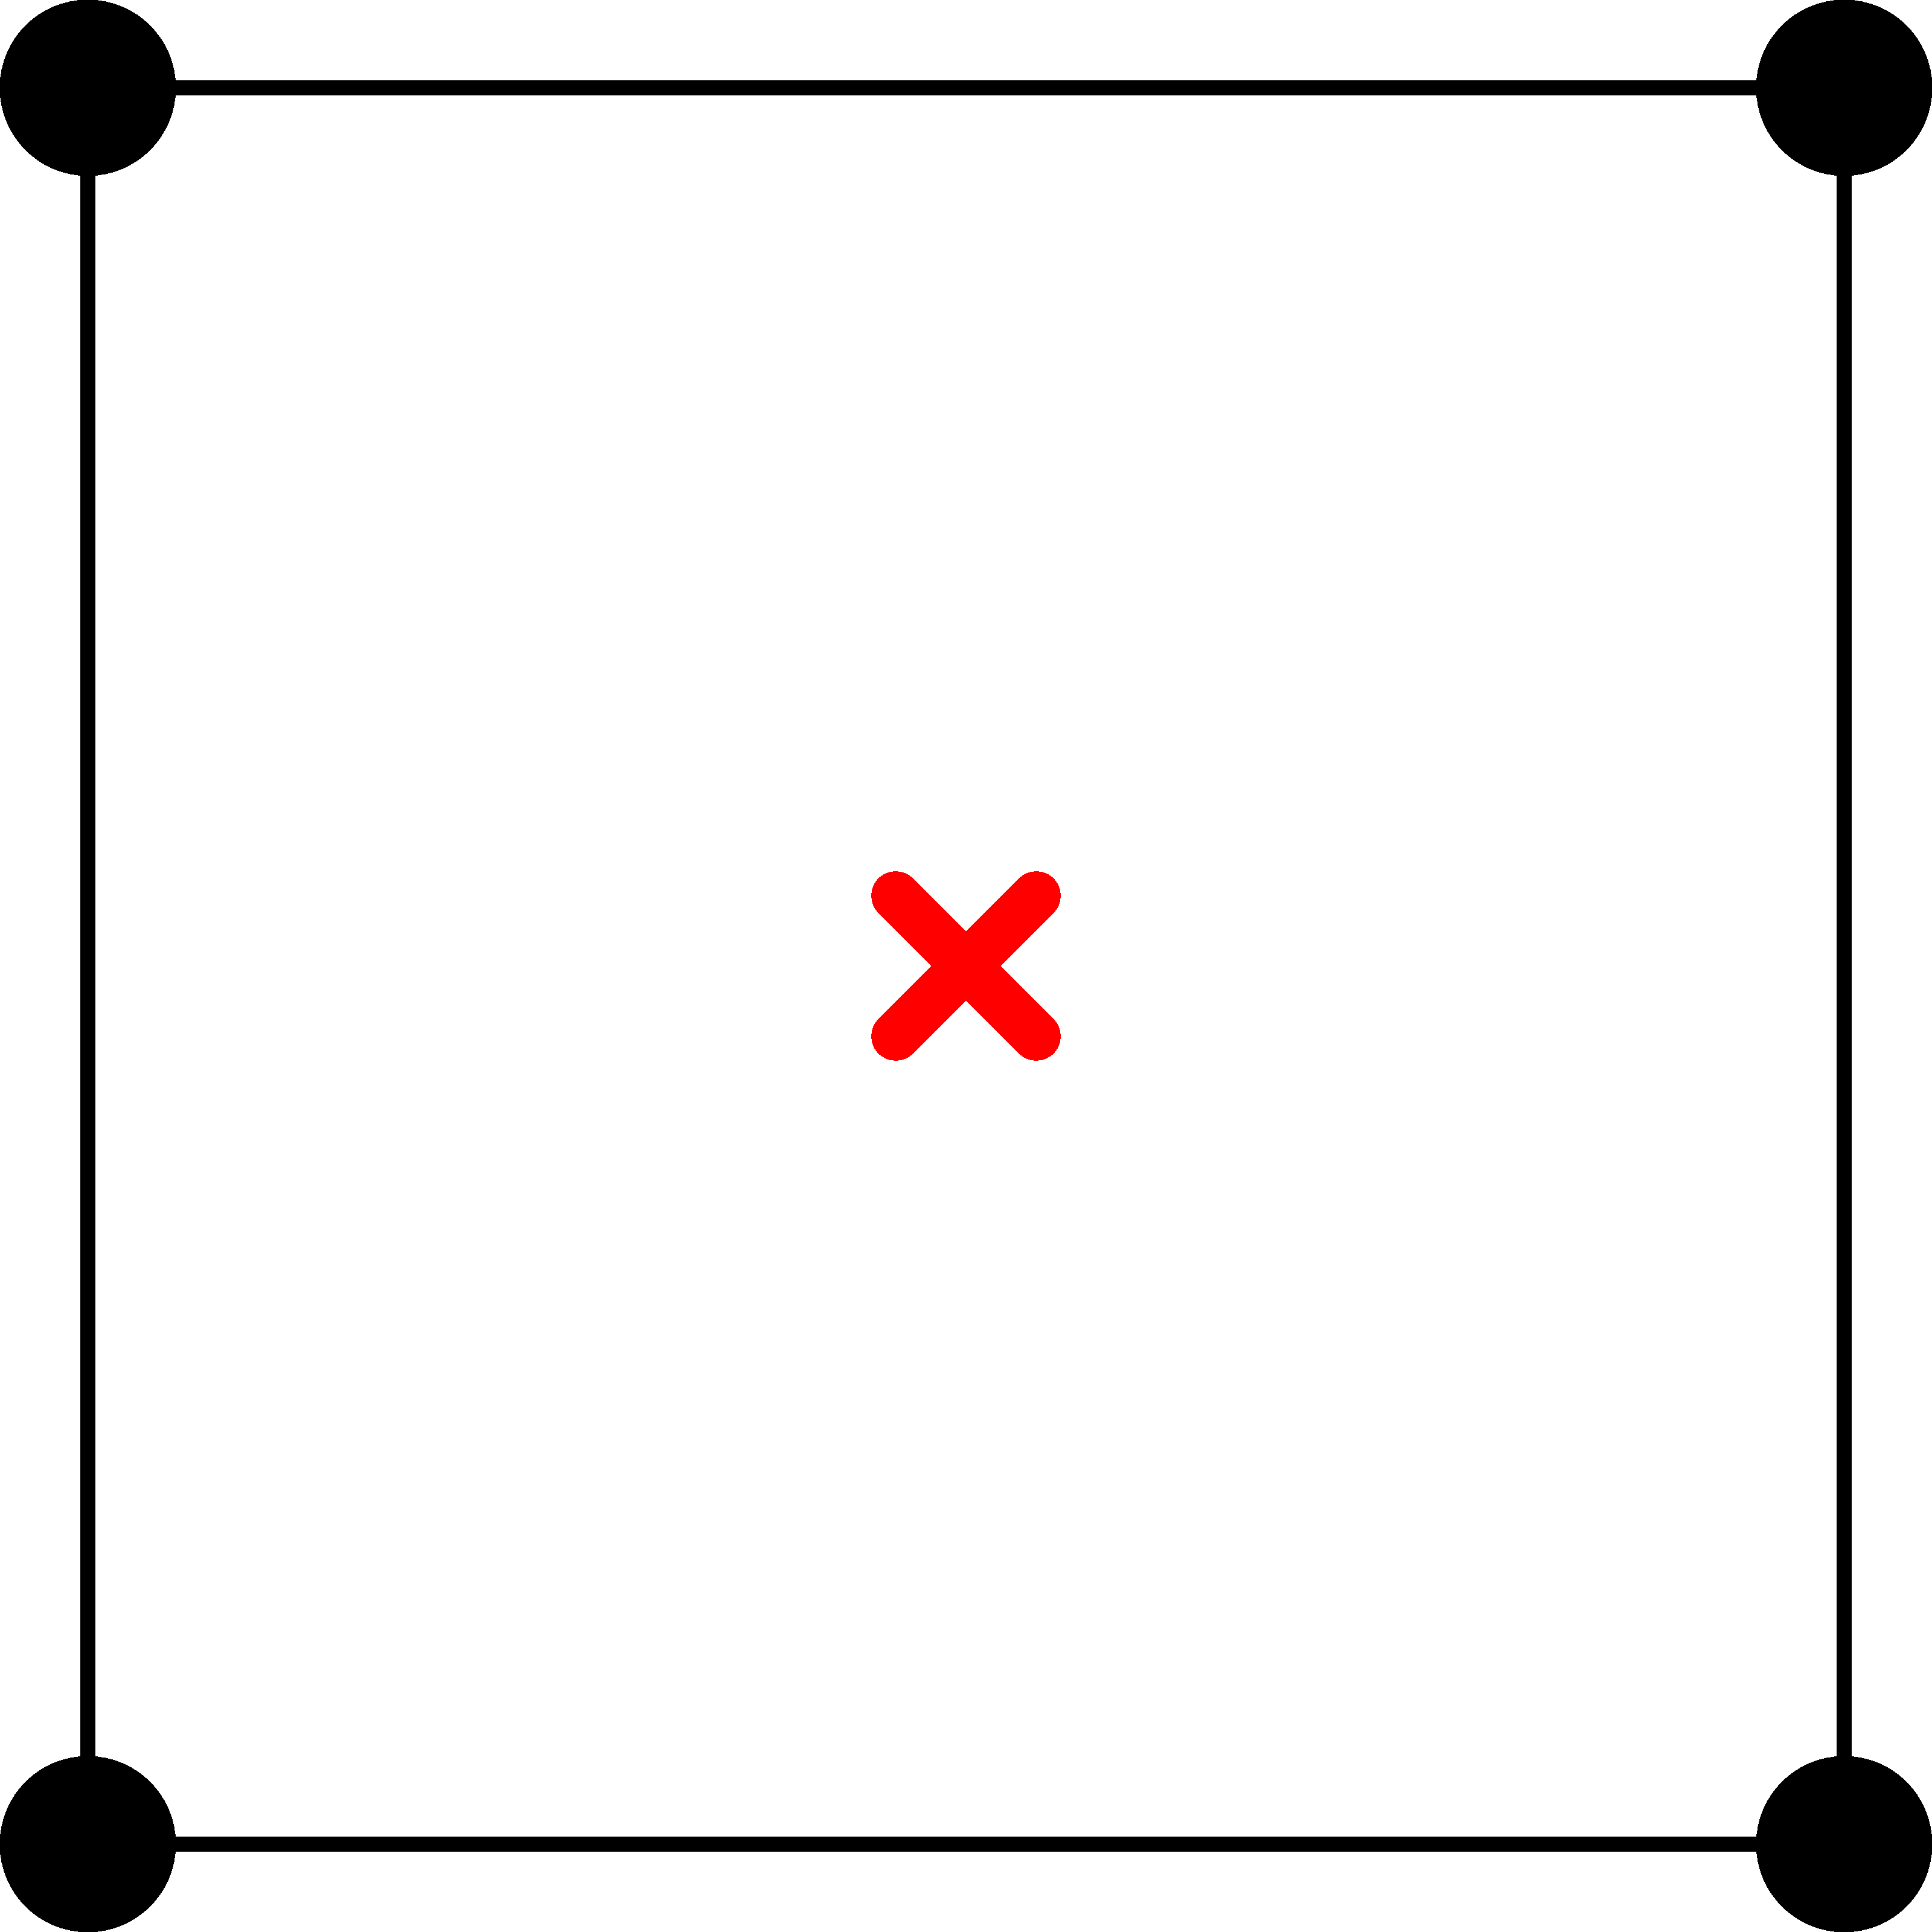
\includegraphics[width=0.3\textwidth]{figures/rd_q4r1.png} \\
            完全积分 & 缩减积分 \\
            \raisebox{-0.3\height}{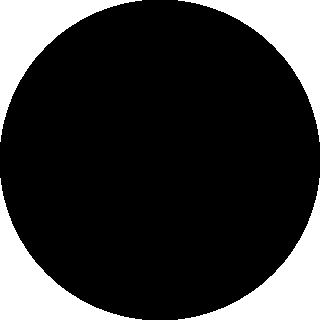
\includegraphics[width=14pt]{figures/legend_u.png}} :位移节点 &
            \raisebox{-0.3\height}{
\includegraphics[width=14pt]{figures/legend_i.png}} :高斯积分点 
        \end{tabular}
        \caption{Quad4单元缩减积分方案}\label{reduced}
\end{figure}

TODO
相反,为保证整体刚度矩阵的正定性,…… 

由上述例子可知,缩减积分方案通过减少体积刚度矩阵离散单元的积分点数量,减少了体积约束自由度,缓解体积自锁现象。但是低阶高斯积分将伴随着数值积分精度不足,引起数值计算结果振荡和精度下降。

\subsection{拉格朗日乘子法与混合离散方案}
施加约束的方式除了传统罚函数法外,常用的方法还有拉格朗日乘子法。
对于体积自锁问题,将压力$p$作为拉格朗日乘子独立变量,可以得到拉格朗日乘子型体积约束施加方案,相对应的强形式中增加了压力$p$与体积应变$\nabla \cdot \boldsymbol u$之间的约束:
\begin{equation}\label{strong_mix}
    \begin{cases}
        \nabla \cdot \boldsymbol \sigma + \boldsymbol b = \boldsymbol 0 & \mathrm{in} \; \Omega \\
        \frac{p}{\kappa} + \nabla \cdot \boldsymbol u = 0 & \mathrm{in} \; \Omega \\
        \boldsymbol \sigma \cdot \boldsymbol n = \boldsymbol t & \mathrm{on} \; \Gamma_t \\
        \boldsymbol u = \boldsymbol g & \mathrm{on} \; \Gamma_g \\
    \end{cases}
\end{equation}
式中应力张量$\boldsymbol \sigma$采用两个变量表示:
\begin{equation}\label{stress_mix}
    \boldsymbol \sigma(\boldsymbol u, p) = p \boldsymbol 1 + 2\mu \boldsymbol \varepsilon^d(\boldsymbol u)
\end{equation}
其中$p\in Q$,$Q = \{q \in L^2(\Omega) \vert \int_{\Omega} q d\Omega = 0\}$。此时,能量泛函具有位移$\boldsymbol u$压力和$p$两个变量,分别对两变量进行变分,可得相对应的伽辽金弱形式为:
位移$\boldsymbol u \in V$, 压力$p \in Q$满足
\begin{equation}\label{weak_mix}
    \begin{aligned}
        a(\delta \boldsymbol u, \boldsymbol u) + b(\delta \boldsymbol u, p) &= f(\delta \boldsymbol u) \quad &\forall \delta \boldsymbol u \in V \\
        b(\boldsymbol u, q) &= \boldsymbol 0 \quad &\forall q \in Q
    \end{aligned}
\end{equation}
式中,$a: V\times V\rightarrow \mathbb R$,$b: V\times Q\rightarrow \mathbb R$ 为双线性算子, $f: V \rightarrow \mathbb R$ 为线性算子,它们具有以下形式:
\begin{align}
    a(\delta \boldsymbol u, \boldsymbol u) &= \int_\Omega \nabla^s \delta \boldsymbol u: \nabla^s \boldsymbol u d\Omega \\
    b(\delta \boldsymbol u, p) &= \int_\Omega \nabla \cdot \delta \boldsymbol u p d\Omega \\
    f(\delta \boldsymbol u) &= \int_{\Gamma_t} \delta \boldsymbol u \cdot \boldsymbol t d\Gamma + \int_{\Omega} \delta \boldsymbol u \cdot \boldsymbol b d\Omega
\end{align}

采用伽辽金法进行求解时,位移$\boldsymbol u$和压力$p$双变量可以采用不同的离散方式进行近似,形成混合离散框架。
近似的位移$u_h$和压力$p_h$及其变分可表示为:
\begin{equation}\label{u_h_mix}
    \boldsymbol u_h(\boldsymbol x) = \sum_{I=1}^{n_u} N_I(\boldsymbol x) \boldsymbol u_I, \quad
    \delta \boldsymbol u_h(\boldsymbol x) = \sum_{I=1}^{n_u} N_I(\boldsymbol x) \delta \boldsymbol u_I
\end{equation}
\begin{equation}\label{p_h_mix}
    p_h(\boldsymbol x) = \sum_{K=1}^{n_p} \Psi_K(\boldsymbol x) p_K, \quad
    \delta p_h(\boldsymbol x) = \sum_{K=1}^{n_p} \Psi_K(\boldsymbol x) \delta p_K
\end{equation}
式中,$n_p$分别为压力节点的总数,$p_K$为压力节点系数,$\Psi_K$为离散$p_h$的形函数。

根据$\delta \boldsymbol  u_h$和$\delta p_h$的任意性,式\eqref{weak_mix}可得到如下离散控制方程:
\begin{equation}\label{equilibrium_mix}
    \begin{bmatrix}
        \boldsymbol K^{uu} & \boldsymbol K^{up} \\ (\boldsymbol K^{up})^{\mathrm T} & \boldsymbol K^{pp}
    \end{bmatrix}
    \begin{Bmatrix}
        \boldsymbol d^u \\ \boldsymbol d^p 
    \end{Bmatrix} =
    \begin{Bmatrix}
        \boldsymbol f \\ \boldsymbol 0 
    \end{Bmatrix}
\end{equation}
式中,$\boldsymbol K^{uu} = \boldsymbol K^d$, $\boldsymbol{K}^{up}$为刚度矩阵中和位移、压力都有关的部分。$\boldsymbol{K}^{pp}$为刚度矩阵中只和压力相关的部分,其分量分别为:
\begin{equation}
    \boldsymbol{K}^{up}_{I J}=\int_{\Omega} \boldsymbol B_{I}^{\mathrm T} \Psi_{J} {d} \Omega
\end{equation}
\begin{equation}  
    \boldsymbol{K}^{pp}_{IJ}=-\frac{1}{\kappa}\int_{\Omega}  \Psi^\mathrm{T}_{I}  \Psi_{J}d\Omega
\end{equation}

为统计约束的自由度个数,将离散控制方程式\eqref{equilibrium_mix}进行变换。
由式\eqref{equilibrium_mix}可将$\boldsymbol d^p$采用$\boldsymbol d^u$表示:
\begin{equation}
    \boldsymbol d^p = (\boldsymbol K^{pp})^{-1} (\boldsymbol K^{up})^{\mathrm T} \boldsymbol d^u
\end{equation}

将上式代入到式\eqref{equilibrium_mix}的第一式中可得:
\begin{equation}\label{equilibrium_projection}
    \begin{split}
        &(\underbrace{\boldsymbol K^{uu}}_{\boldsymbol K^d} +  \underbrace{\boldsymbol K^{up}(\boldsymbol K^{pp})^{-1}(\boldsymbol K^{up})^{\mathrm T}}_{\tilde{\boldsymbol K}^v}) \boldsymbol d^u = \boldsymbol f \\
        \Rightarrow\;& (\boldsymbol K^d + \tilde{\boldsymbol K}^v) \boldsymbol d^u= \boldsymbol f
    \end{split}
\end{equation}

为保证积分精度,混合离散方案均采用完全积分进行数值积分,且考虑离散控制方程\eqref{equilibrium_mix}中整体刚度矩阵的正定性,$\boldsymbol K^{uu}$、$\boldsymbol K^{pp}$为满秩矩阵。因此,结合式\eqref{equilibrium_projection}可得混合离散方案中的位移自由度$\mathit{rank}(\boldsymbol K^d)$、压力自由度$\mathit{rank}(\tilde{\boldsymbol K}^v)$分别为:
\begin{equation}
    \mathit{rank}(\boldsymbol K^d)=n_d\times n_u
\end{equation}
\begin{equation}
    \mathit{rank}(\tilde{\boldsymbol K}^v)=\text{min}(\mathit{rank}({\boldsymbol K}^{up}),\mathit{rank}({\boldsymbol K}^{pp}))=n_p
\end{equation}

以图\ref{mix_ex}所示的常用于免自锁的Q4P1单元混合离散方案为例,Q4P1单元由四个位移节点和一个压力节点组成。图中单个单元的位移自由度为:
\begin{equation}
    \mathit{rank}(\boldsymbol K^d)=2\times 4=8
\end{equation}
压力自由度为:
\begin{equation}
    \mathit{rank}(\tilde{\boldsymbol K}^v)=1
\end{equation}
\begin{figure}[!ht]
    \centering
        \begin{tabular}{c@{\hspace{24pt}}c}
            \multicolumn{2}{c}{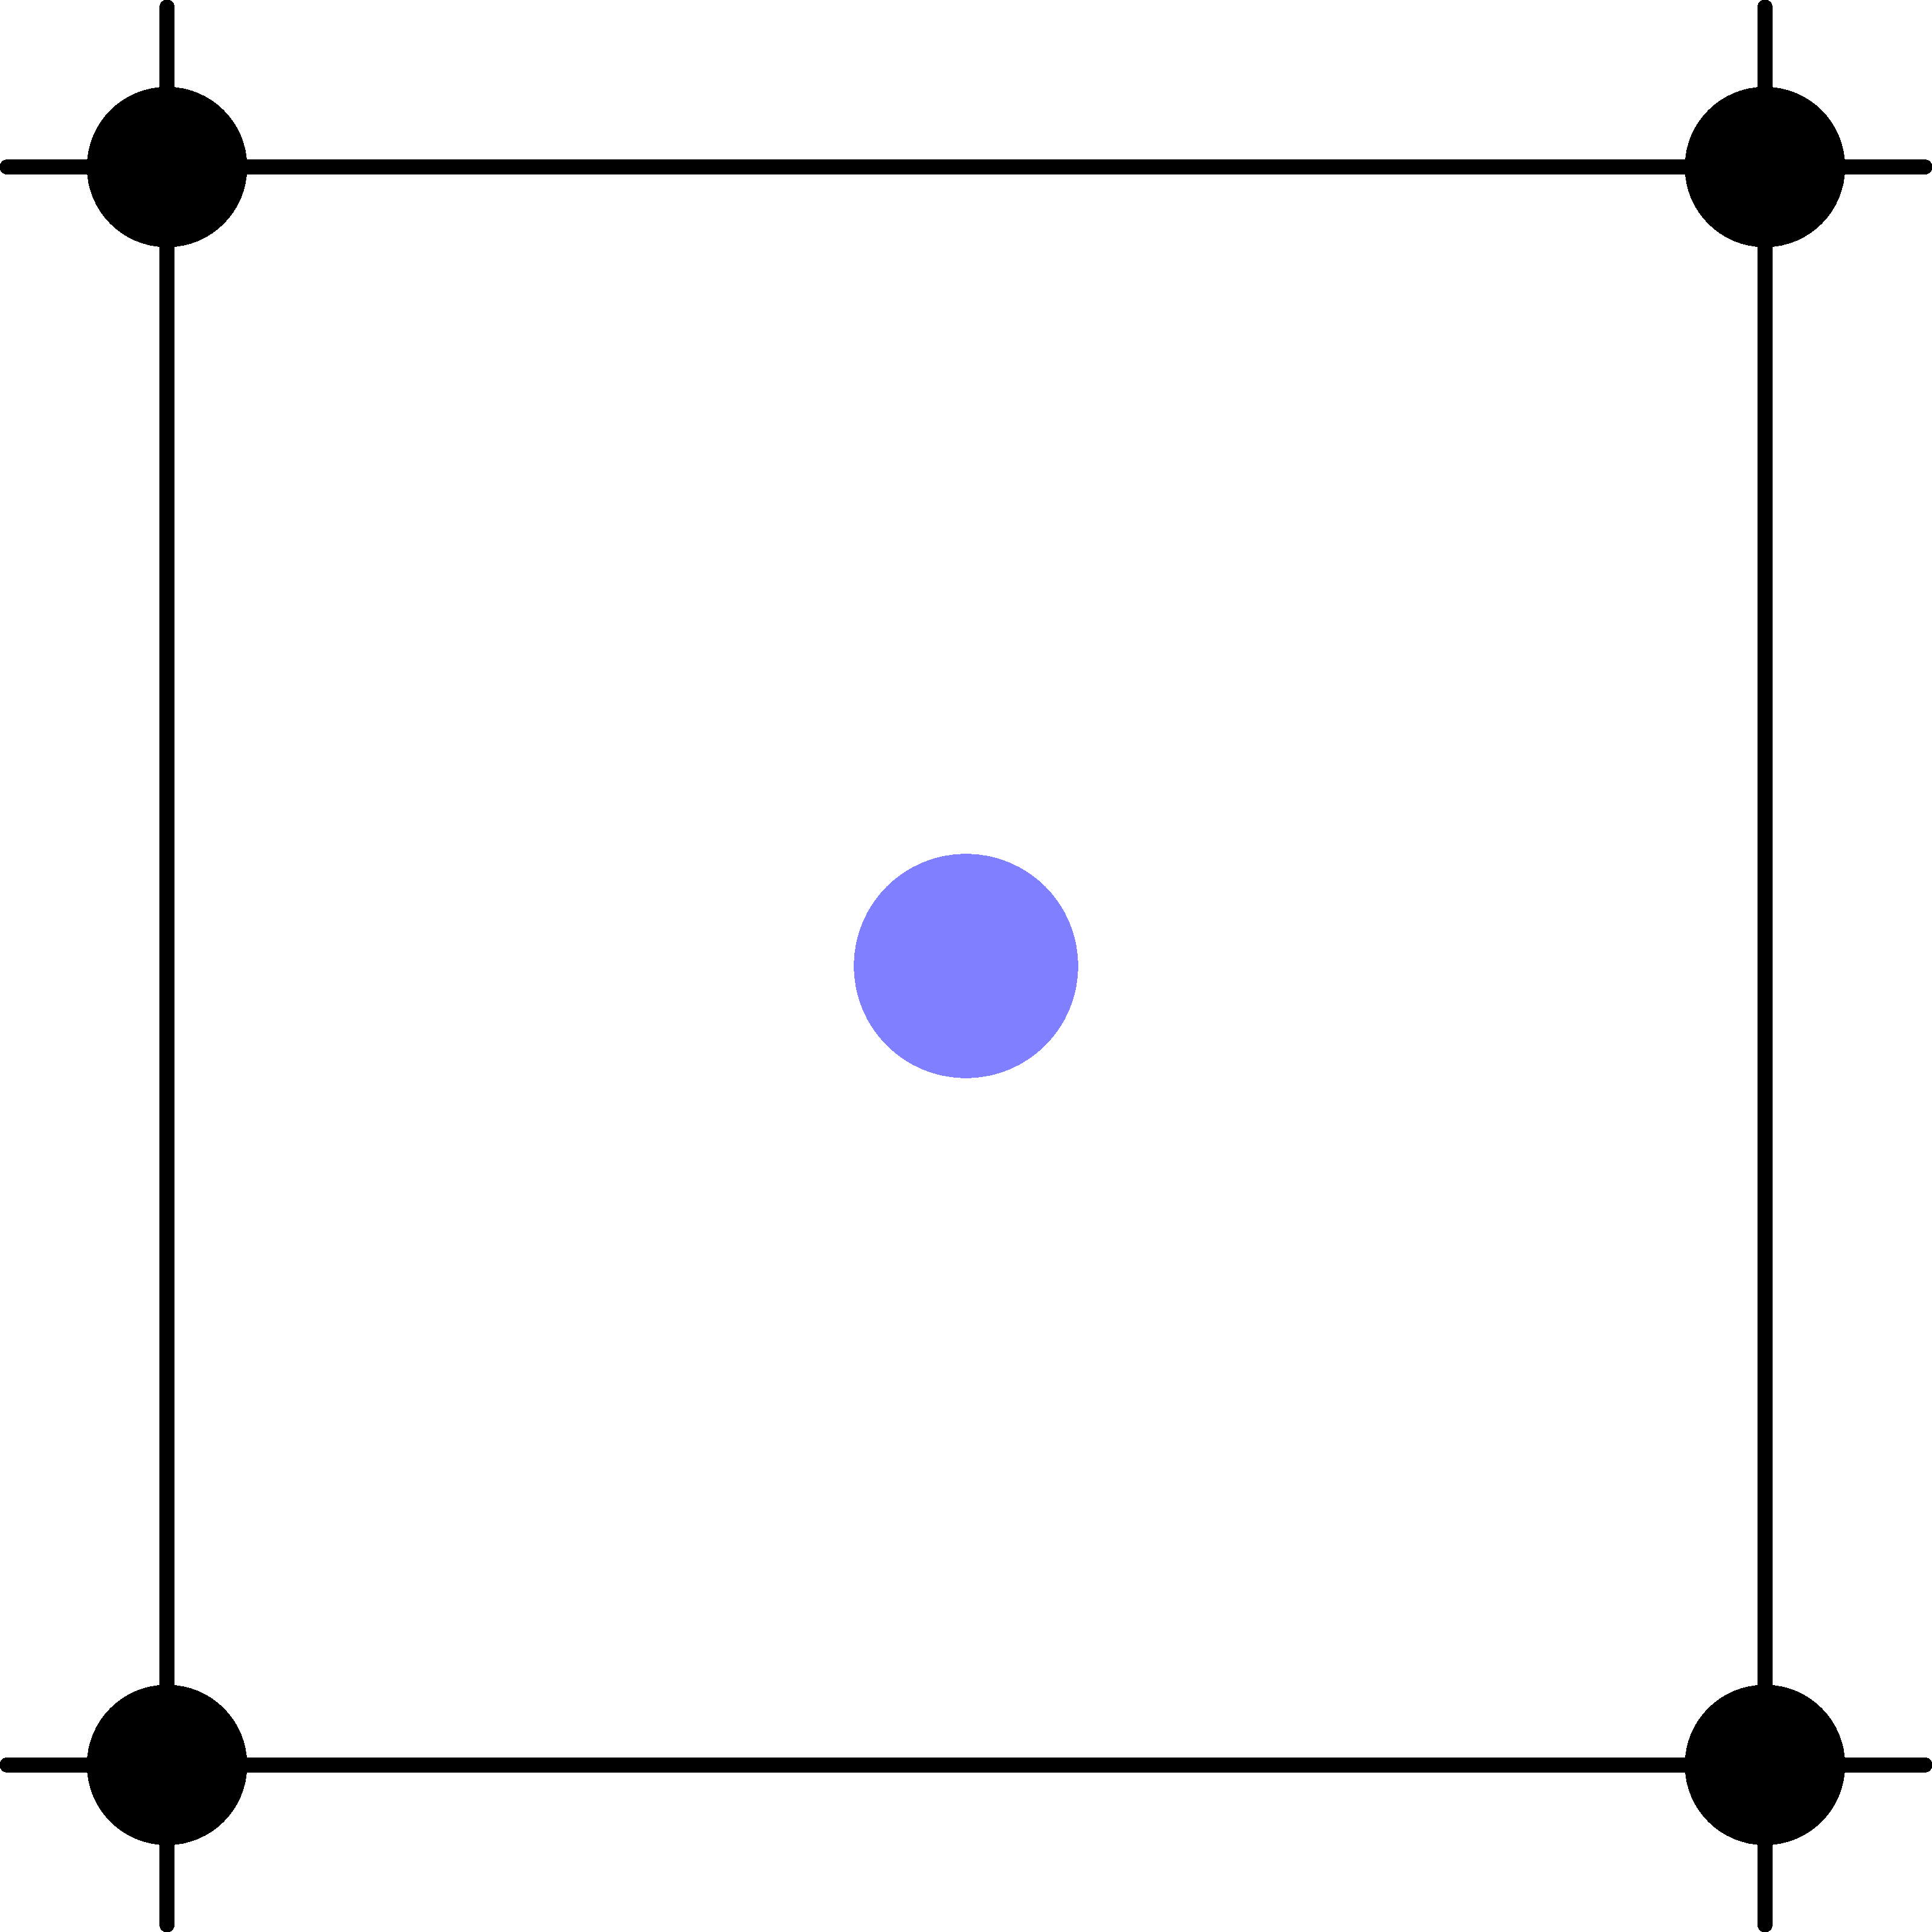
\includegraphics[width=0.3\textwidth]{figures/mix_Q4P1.png}}\\
            \raisebox{-0.3\height}{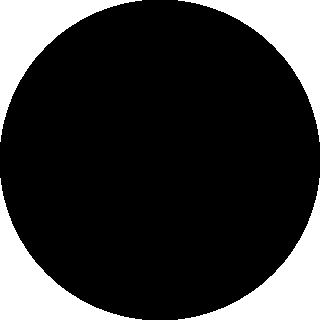
\includegraphics[width=14pt]{figures/legend_u.png}} :位移节点 &
            \raisebox{-0.3\height}{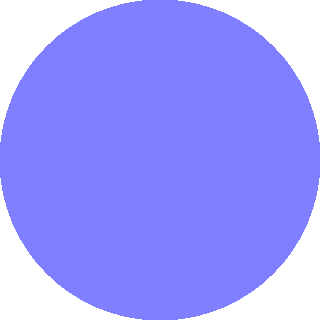
\includegraphics[width=14pt]{figures/legend_p.png}} :压力节点 
        \end{tabular}
    \caption{Q4P1单元混合离散方案}\label{mix_ex}
\end{figure}

由上述例子可知,混合离散方案依附单元布置不同的位移节点和压力节点,减少了压力节点的数量从而减少了位移自由度的个数,缓解体积自锁现象。
\subsection{罚函数法和拉格朗日乘子法方法的等价性}
由上述小节可知,罚函数型和拉格朗日乘子型缓解体积自锁方案均可以达到相类似的效果,两者也可通过数值积分法的等效投影证明两类方法的等价性。
从拉格朗日乘子法的离散方程\eqref{equilibrium_projection}第二式中可以看出,压力$p_h$的解是$3\kappa \nabla \cdot \boldsymbol u_h$的一个正交投影。
令$\mathcal P_h$为正交投影算子,满足:
\begin{equation}\label{ch_2:eq:orthogonal}
    (q_h,\mathcal P_h \boldsymbol u_h) = (q_h, \nabla \cdot \boldsymbol u_h), \quad \forall q_h \in Q_h
\end{equation}
其中,$(\bullet,\bullet)$为内积算子。
为表示方便,可将投影后的位移散度写作$p_h=\mathcal P_h \boldsymbol u_h = \tilde \nabla \cdot \boldsymbol u_h$。且有$\tilde \nabla \cdot \boldsymbol u_h \in \mathrm{Im} \mathcal P_h$,其中$\mathrm{Im} \mathcal P_h \in Q_h$为$\mathcal P_h$的相空间\cite{philippeg.2013}。
此时,式\eqref{ch_2:eq:orthogonal}可改写为:
\begin{equation}
    \int_\Omega q_h(\nabla \cdot \boldsymbol u_h - \tilde \nabla \cdot \boldsymbol u_h) d\Omega = 0, \quad \forall q_h \in Q_h
\end{equation}
将上式代入弱形式\eqref{equilibrium_mix}中,其主应力部分可转化为:
\begin{equation}\label{projection_mixed}
    \begin{split}
        \int_\Omega \nabla \cdot \delta \boldsymbol u_h p_h d\Omega &= \underbrace{\int_\Omega (\nabla \cdot \delta  \boldsymbol u_h - \tilde \nabla \cdot \delta \boldsymbol u_h) p_h d\Omega}_0 + \int_\Omega \tilde \nabla \cdot \delta \boldsymbol u_h \underbrace{p_h}_{\tilde \nabla \cdot \boldsymbol u_h} d\Omega \\
        &= \int_\Omega 3\kappa \tilde \nabla \cdot \delta \boldsymbol u_h \tilde \nabla \cdot \boldsymbol u_h d\Omega \\
    \end{split}
\end{equation}
里兹--伽辽金变分方程变为:
位移$\boldsymbol u_h \in V_h$满足
\begin{equation}
    \int_\Omega 2\mu \delta \boldsymbol \varepsilon^d_h : \boldsymbol \varepsilon^d_h d\Omega +
    \int_\Omega 3\kappa \tilde \nabla \cdot \delta \boldsymbol u_h \tilde \nabla \cdot \boldsymbol u_h d\Omega =
    \int_{\Gamma_t} \delta \boldsymbol u_h \cdot \boldsymbol t d\Gamma + \int_\Omega \delta \boldsymbol u_h \cdot \boldsymbol b d\Omega, \quad \forall \boldsymbol u_h \in V_h
\end{equation}

与此同时对于罚函数法,数值积分也可以被视作一种投影。设$\varrho_i$为正交多项式满足:
\begin{equation}
    \int_{\Omega_C} \varrho_i \varrho_j d\Omega = 
    \begin{cases}
        w_i  & i = j \\
        0 & i \ne j
    \end{cases}
\end{equation}
正交插值 $\mathcal T^{k}: V_h \rightarrow W^{k}$,其中 $W^{k}$ 是由$k$个正交多项式构成的插值空间:
\begin{equation}
    W^{k}:= \mathrm{span}\{\varrho_i \}_{i=1}^{k}
\end{equation}
对于传统高斯积分方案,$\varrho_i(\boldsymbol x_j) = \delta_{ij}$, $\boldsymbol x_j$是积分点的位置。体积应变可以通过正交插值法表示为:
\begin{equation}
    \nabla \cdot \boldsymbol u_h(\boldsymbol x) \approx \bar \nabla \cdot \boldsymbol u_h(\boldsymbol x) = \sum_{G=1}^{n_g} \varrho_G(\boldsymbol x) \nabla \cdot \boldsymbol u_h(\boldsymbol x_G), \quad \nabla \cdot \boldsymbol u_h(\boldsymbol x_G) = \bar \nabla \cdot \boldsymbol u_h(\boldsymbol x_G)
\end{equation}
而积分点被视为插值系数。虽然积分点的总数$n_g$低于完全积分,这意味着 $\nabla \cdot \boldsymbol u_h$ 投影到子空间。
\begin{equation}\label{projection_penalty}
    \begin{split}
        \int_\Omega 3\kappa \nabla \cdot \delta \boldsymbol u_h \nabla \cdot \boldsymbol u_h d\Omega
        &= \sum_{C=1}^{n_e} \sum_{G,L=1}^{n_g} 3\kappa \nabla \cdot \delta \boldsymbol u_h(\boldsymbol x_G) \nabla \cdot \boldsymbol u_h(\boldsymbol x_L) \int_\Omega \varrho_G \varrho_L d\Omega  \\
        &= \sum_{C=1}^{n_e} \sum_{G=1}^{n_g} 3\kappa \nabla \cdot \delta \boldsymbol u_h(\boldsymbol x_G) \nabla \cdot \boldsymbol u_h(\boldsymbol x_G) J_C w_G \\
    \end{split}
\end{equation}

通过对比式\eqref{projection_penalty}和式\eqref{projection_mixed},罚函数法实际上与拉格朗日乘子法等价,两种方法都可以用投影的方式来描述。
缩减积分方案与混合离散方案调整体积自由度的方法也等价,即$n_g=n_p$

\section{免体积自锁条件}
\subsection{体积约束比}
从上文介绍的两种方法可知,调整体积约束自由度可以免体积自锁。相关的结论Hughes已经做出了总结\cite{hughes2000},并提出了约束比的概念。
约束比是用来衡量变量间的约束程度的重要指标。对于体积不可压问题而言,约束比定义为位移总自由度与压力总自由度的比值。在理想情况下,最优约束比应与相应的偏微分控制方程一致。
\begin{equation}
    r = \frac{n_d\times n_u}{n_p}, \quad 
    \begin{cases}
        r > n_d & \text{过少的约束} \\
        r = n_d & \text{最优} \\
        r < n_d & \text{过多的约束} \\
    \end{cases}
\end{equation}

在二维情况下,不可压问题涉及两个位移控制方程和一个压力控制方程,因此最优约束比为2.当约束比小于2时会出现体积自锁的倾向。当约束比大于2时可能会导致压力计算出现较大误差。
图\ref{pressure_elements}为两个不同的二维单元混合离散方案,图中阴影部分为边界条件,边界上节点自由度均受到约束。

图\ref{pressure_elements}(a)为线性位移--常数压力三角形单元(T3P1),它的约束比为:
\begin{equation}
    r= \frac{2\times n_u}{n_p}=\frac{2\times 1}{2}=1
\end{equation}
表明此单元体积约束过多,会产生体积自锁,与实际情况一致。

图\ref{pressure_elements}(b)为双线性位移--常数压力四边形单元(Q4P1),约束比为:
\begin{equation}
    r= \frac{2\times n_u}{n_p}=\frac{2\times 1}{1}=2
\end{equation}
此单元满足最优约束比,能够缓解体积自锁。
\begin{figure}
    \centering
        \begin{tabular}{c@{\hspace{24pt}}c}
            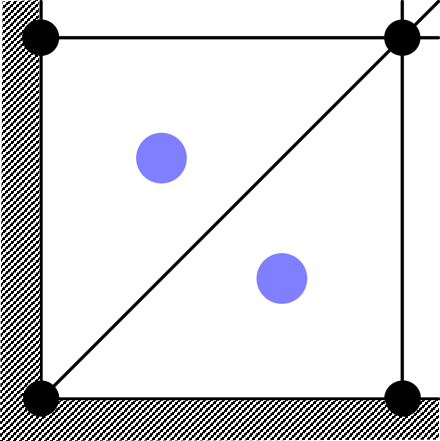
\includegraphics[width=0.3\textwidth]{figures/T3P1.png} &
            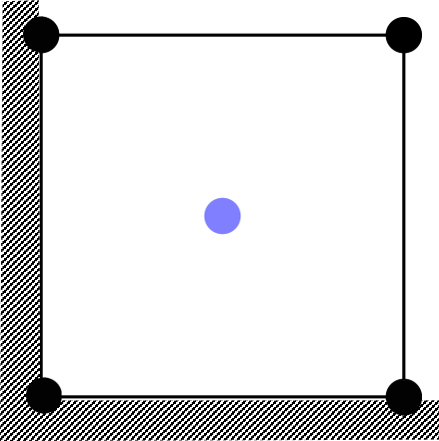
\includegraphics[width=0.3\textwidth]{figures/Q4P1.png} \\
            (a) & (b) \\
            \raisebox{-0.3\height}{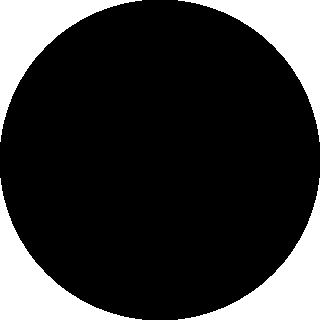
\includegraphics[width=14pt]{figures/legend_u.png}} :位移节点 &
            \raisebox{-0.3\height}{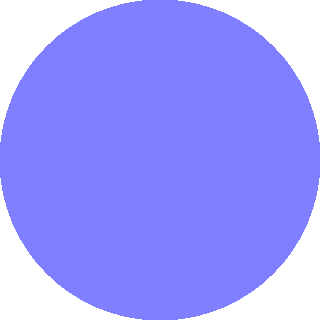
\includegraphics[width=14pt]{figures/legend_p.png}} :压力节点 
        \end{tabular}
        \caption{二维位移压力单元示例}\label{pressure_elements}
    \end{figure}

从上述分析来看,Hughes对约束比的总结只是一种启发式手段,并不能确保单元组合能够缓解自锁现象。它主要作为一种便捷的工具来评估单元是否有缓解自锁的潜在能力,在全面评估单元性能时,还需要综合考虑其它相关因素。
对于具有相同数量位移和压力节点的经典单元,尽管其约束比为最优,但在实际应用中仍会出现体积自锁问题。尽管其它满足最优约束比的单元可以在一定程度上缓解体积自锁现象,但它们并不一定能满足LBB稳定性条件。
例如图\ref{pressure_elements}(b)Q4P1单元就不满足LBB稳定性条件,压力的解出现了明显的振荡现象,这种现象通常被称为伪压力模式或应力棋盘模式。
\subsection{LBB稳定性条件}
Ladyzhenskaya--Babuska--Brezzi(LBB)条件,也被称为inf--sup条件\cite{babuska1997a,bathe1996},是对免自锁方法更为精确的要求。这一条件基于混合离散框架构建,当满足inf--sup条件时,可以确保混合方程的准确性和稳定性。
\begin{equation}\label{infsup}
    \inf_{q_h \in Q_h} \sup_{\boldsymbol v_h \in V_h} \frac{\vert b(q_h,\boldsymbol v_h) \vert}{\Vert q_h \Vert_Q \Vert \boldsymbol v_h \Vert_V} \ge \beta > 0
\end{equation}
其中$\beta$为与单元尺寸$h$无关的常数。

建立特征值问题\cite{chapelle1993}可以数值验证离散方案是否通过满足inf--sup条件。
\begin{equation}\label{eigenvalue}
    \boldsymbol K^d=\lambda\boldsymbol K^v,\quad \beta=\sqrt{\lambda_p}
\end{equation}
式中$\lambda_p$为最小非零特征值。

在理论分析方面,以下解析证明框架\cite{chapelle1993}始终满足inf--sup条件,通过确定离散方案是否包含在该框架内,可以验证其是否满足inf--sup条件。

\begin{equation}\label{analy}
    \begin{cases}
        &\Vert\Pi_1 w\Vert_V \le c_1\Vert w\Vert_W \\
        &b(\Pi_2\nu-\nu,q_h)=0 \quad \forall q_h \in Q_h\\
        &\Vert \Pi_2(I-\Pi_1)w \Vert_V \le c \Vert w\Vert_W \\
    \end{cases}
\end{equation}

表\ref{infsuptest}详细列出了用于体积锁定的经典单元,包括它们的约束比、数值验证以及解析证明结果。显然,传统混合有限元法中使用的单元在约束比最优的情况下无法满足inf-sup条件。相反,满足inf-sup条件的单元通常存在体积约束不足的情况。无论是不满足inf-sup条件还是体积约束不足,都会对结果的准确性和稳定性产生影响。同时,对inf-sup条件的数值验证和解析证明都相当复杂,约束比与inf-sup条件之间的关系也并不明确。
\begin{table}[H]
    \centering
    \renewcommand\arraystretch{1.2}
    \caption{inf-sup条件验证} \label{infsuptest}
    \begin{tabular}{c|c|c|c}
        \hline
        \multirow{2}{*}{离散方案}&\multirow{2}{*}{约束比}&\multicolumn{2}{c}{inf-sup条件}\\
        \cline{3-4}
        & &数值验证&解析证明\\
        \hline
        \begin{tabular}{c}
            \begin{minipage}{0.1\columnwidth}
                \centering
                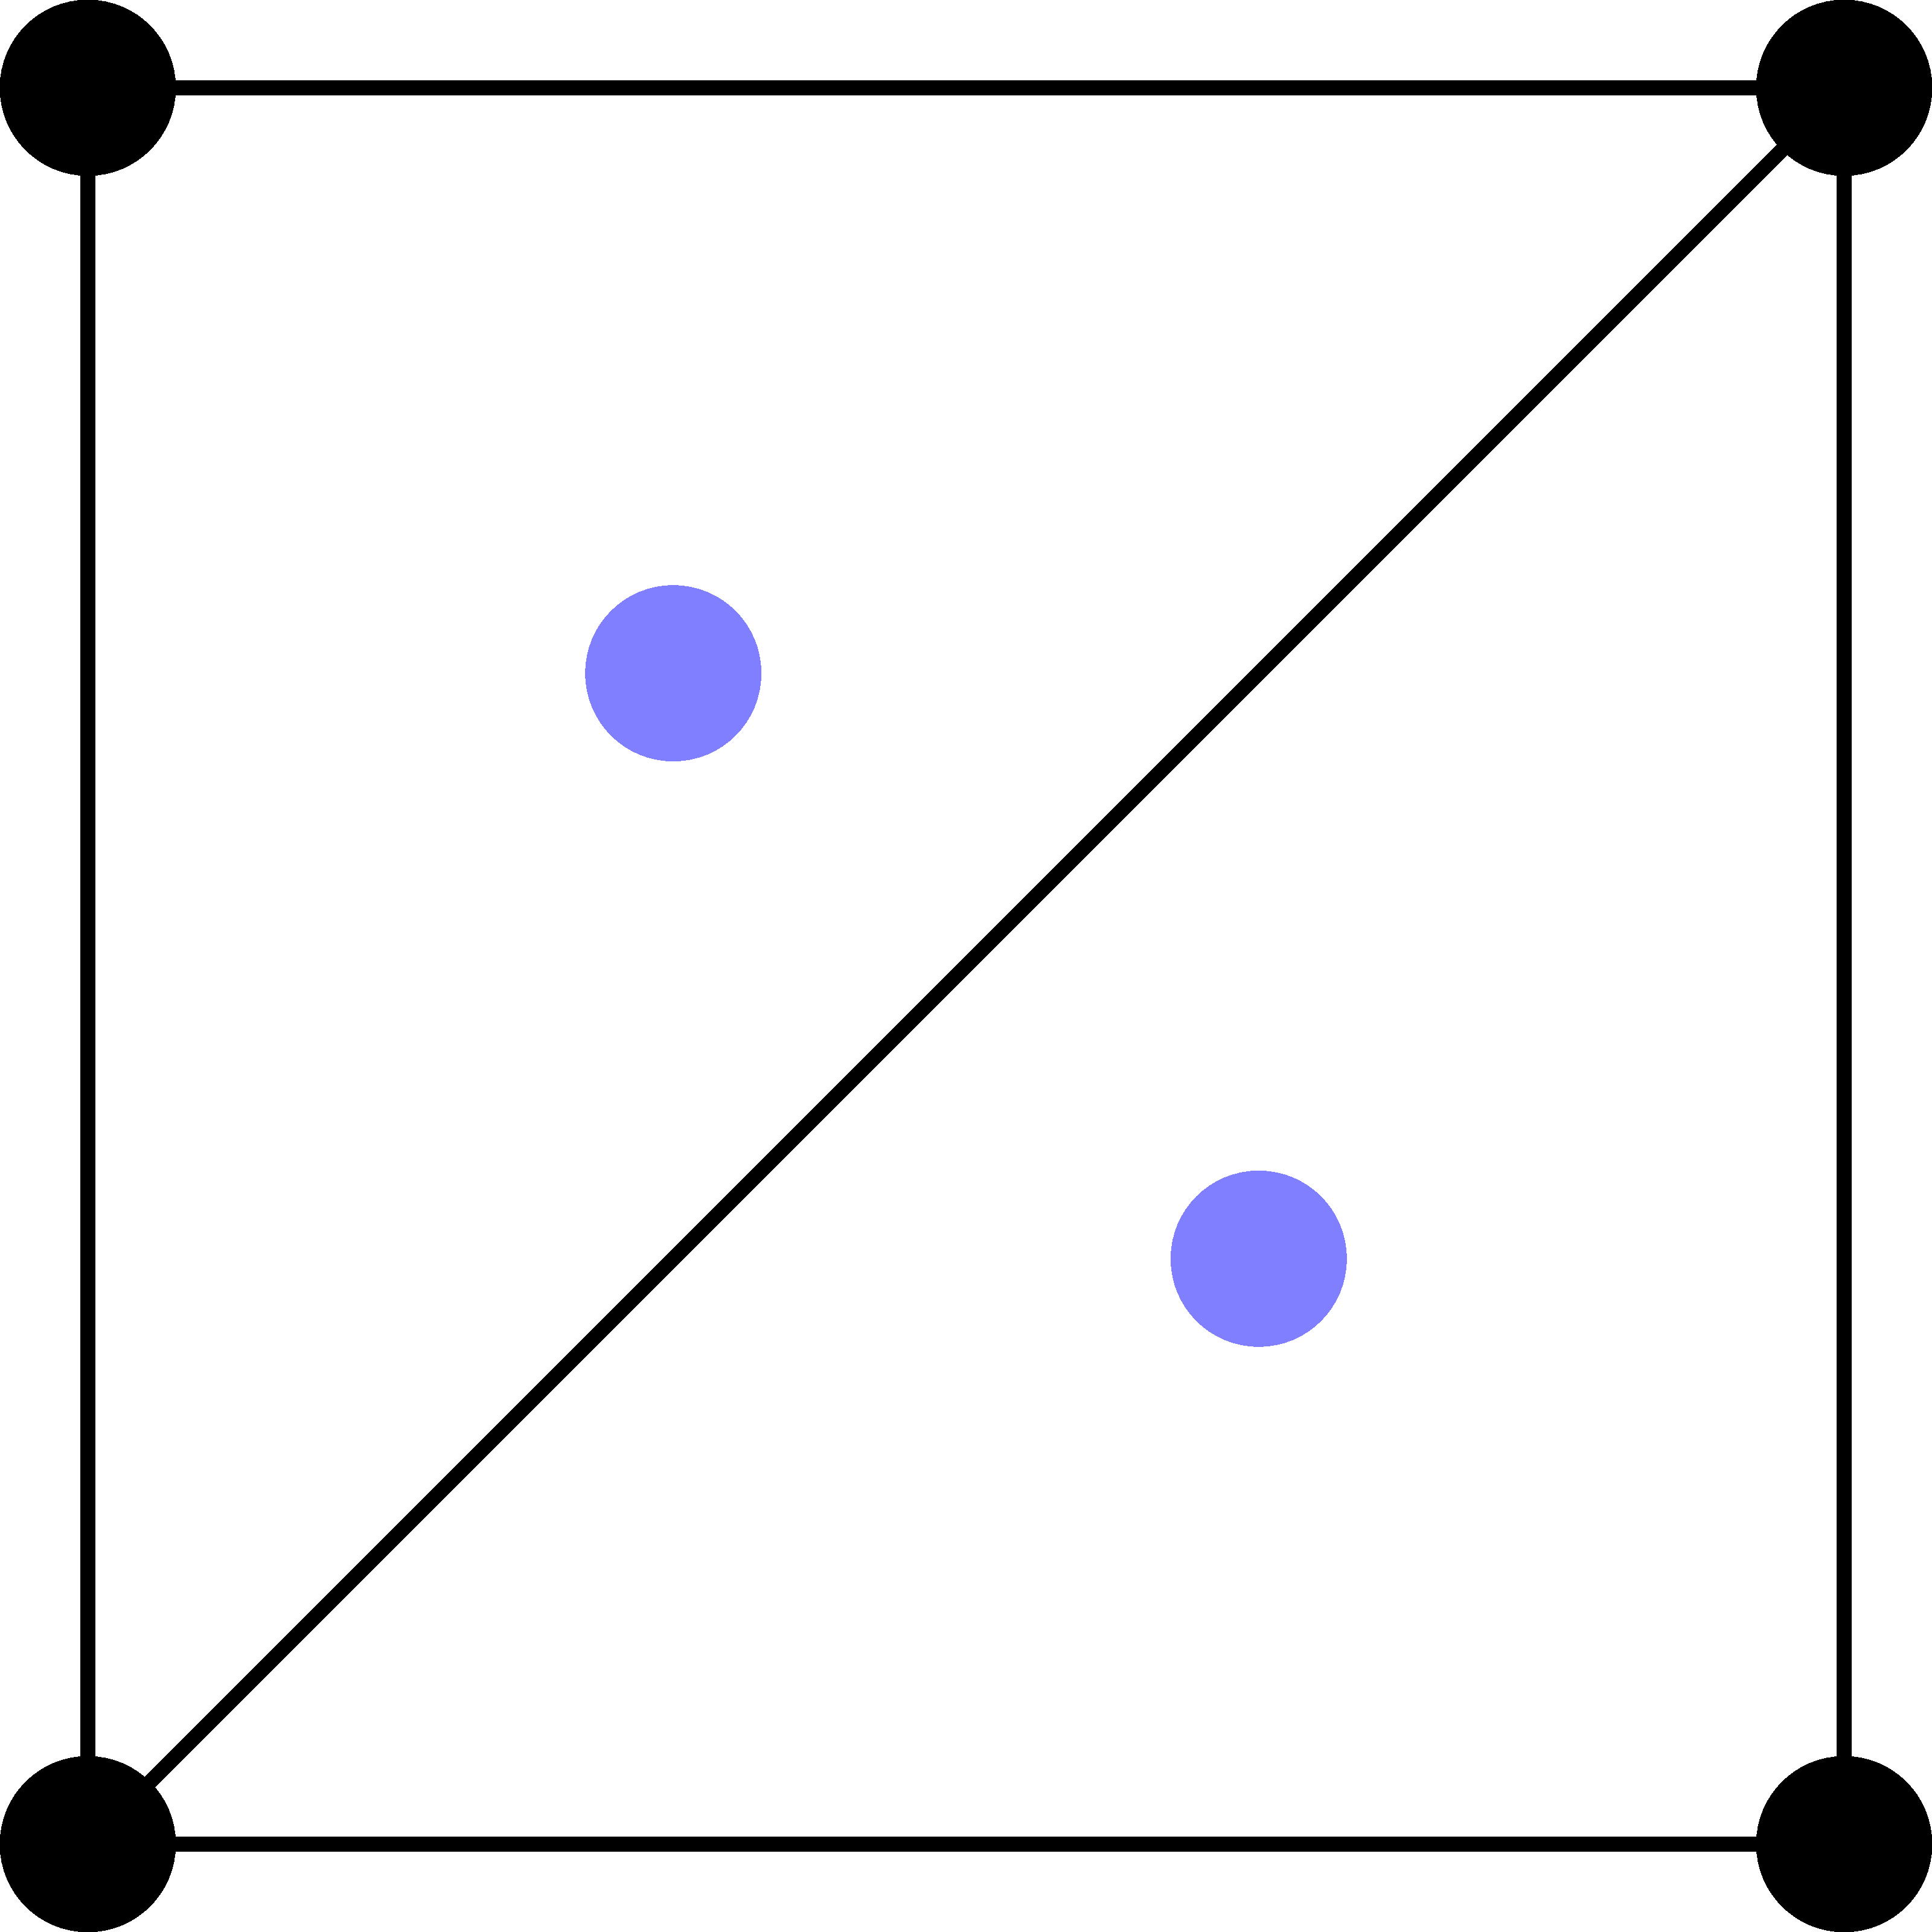
\includegraphics[width=0.9\textwidth]{figures/mix_T3P1.png}
            \end{minipage}\\T3P1
        \end{tabular}
        &1&$\times$ & $\times$\\
        \hline
        \begin{tabular}{c}
            \begin{minipage}{0.1\columnwidth}
                \centering
                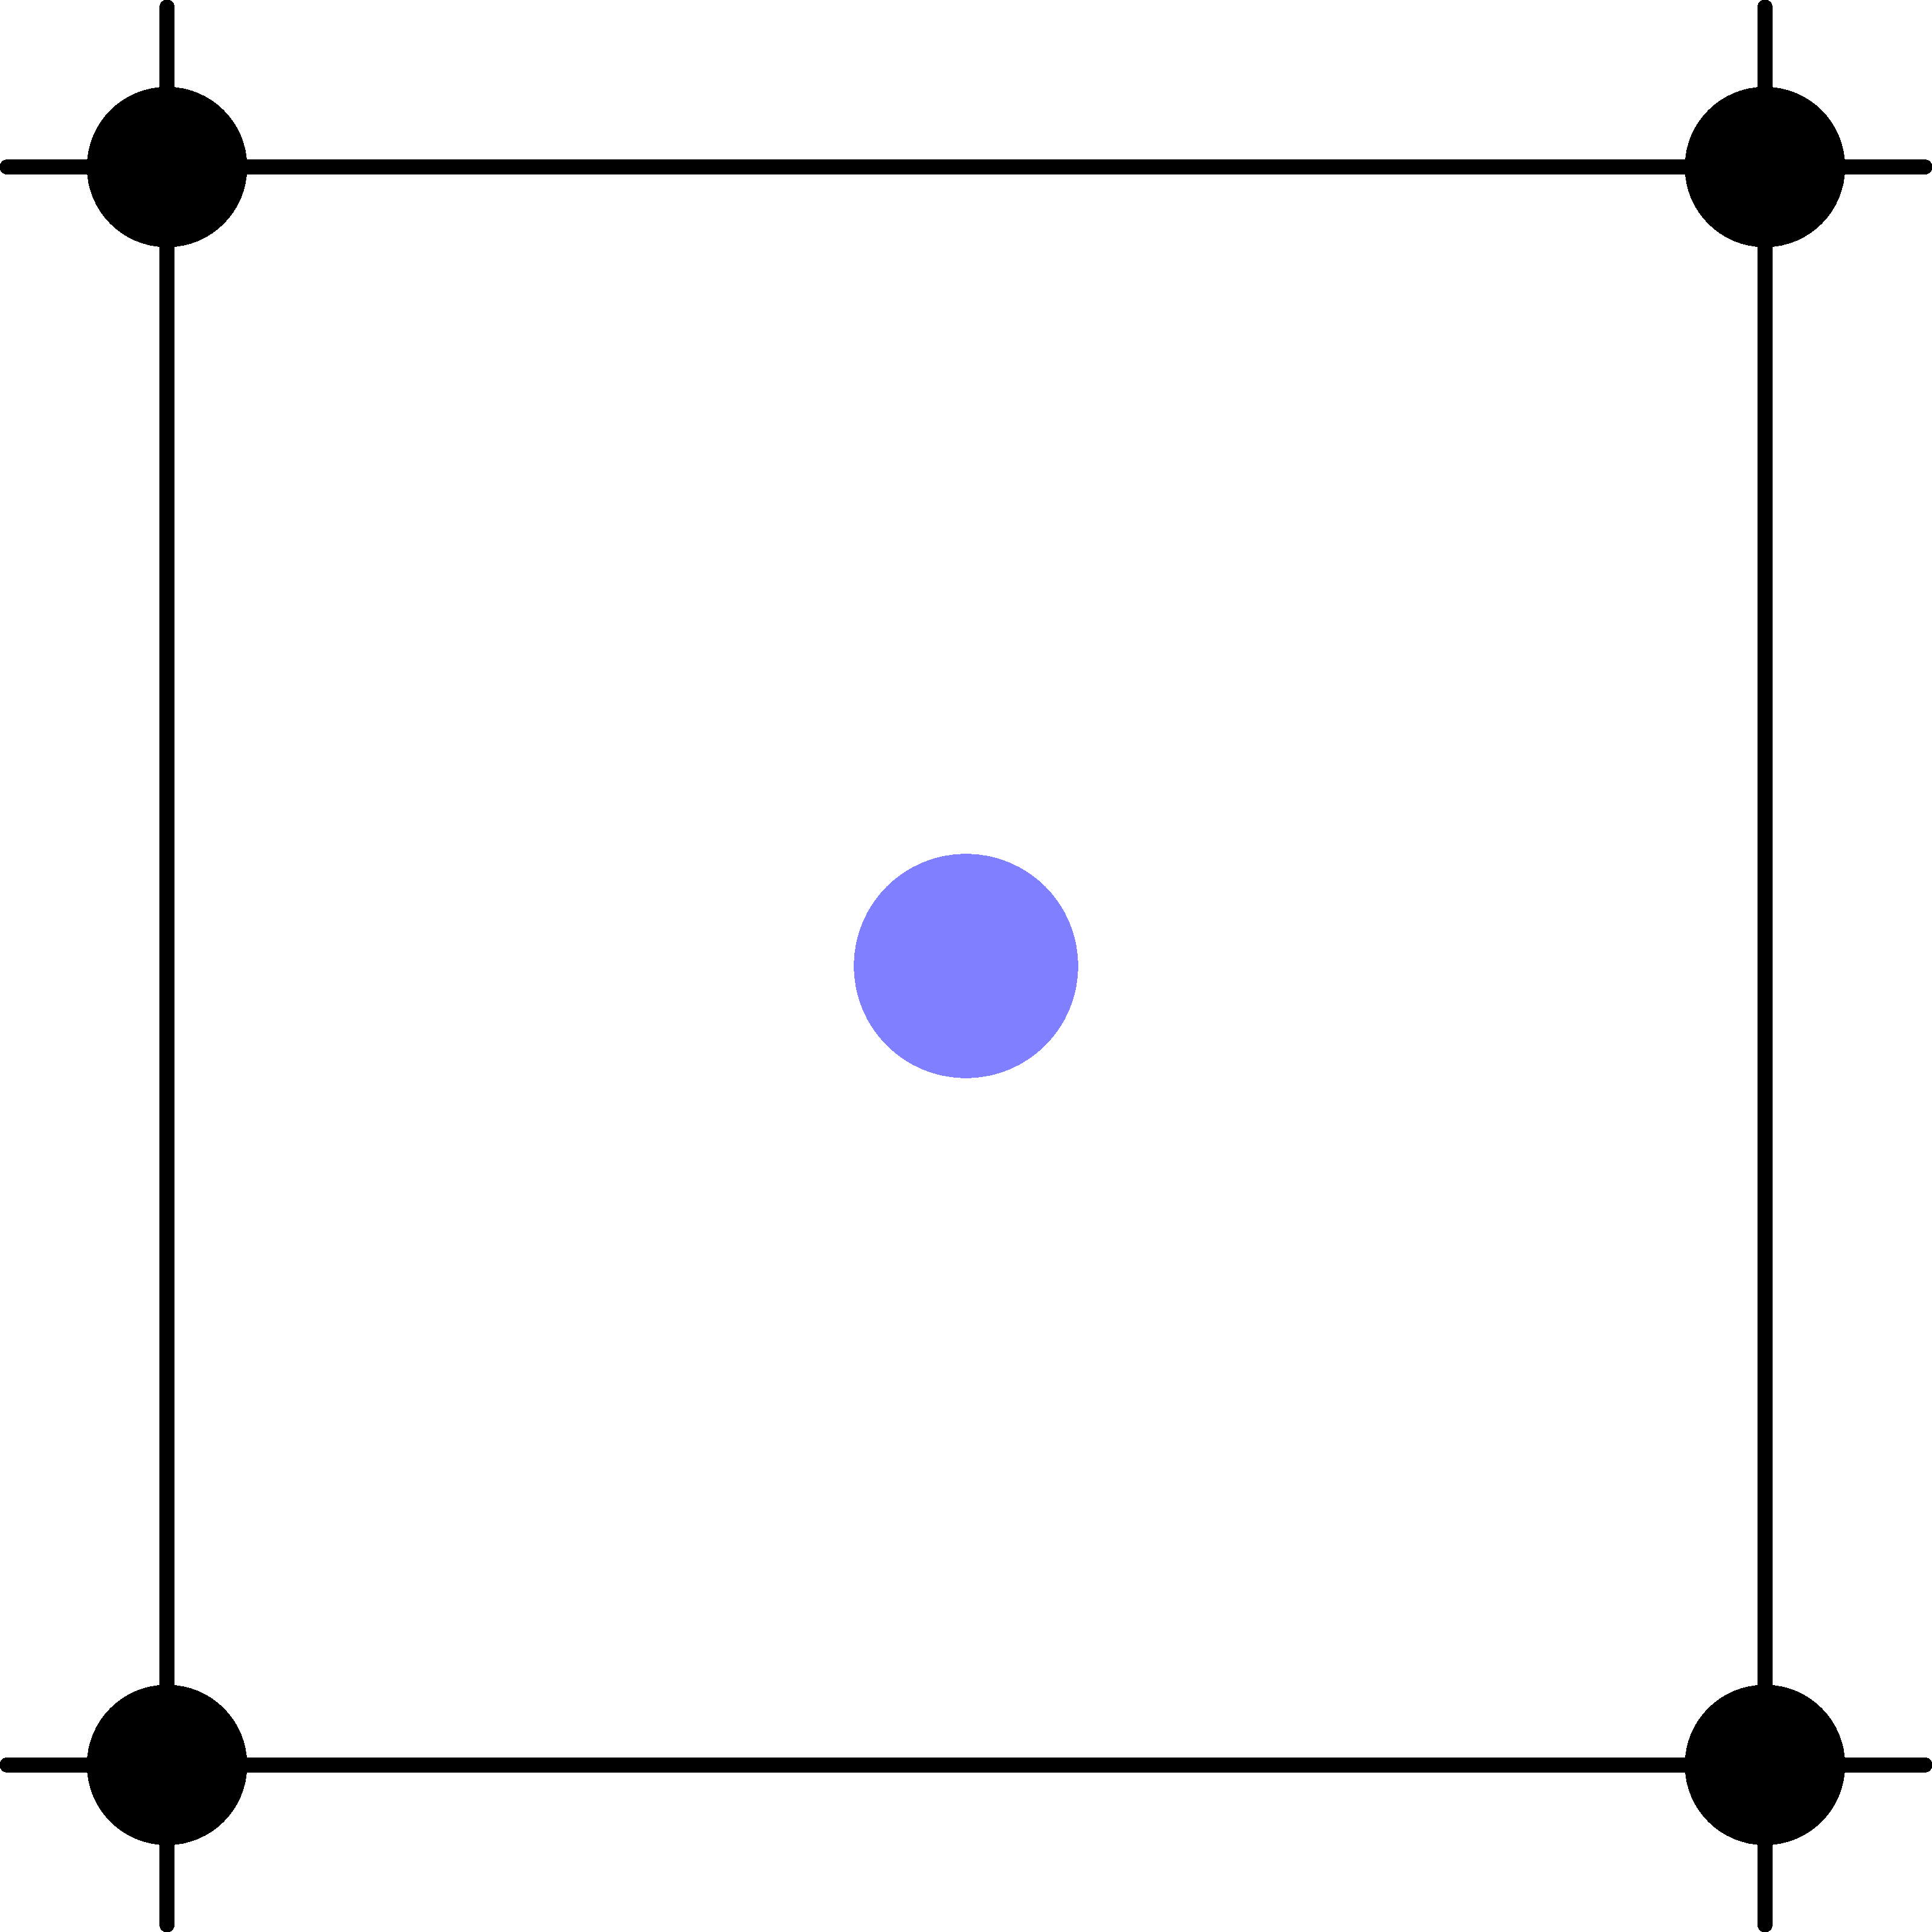
\includegraphics[width=0.9\textwidth]{figures/mix_Q4P1.png}
            \end{minipage}\\Q4P1
        \end{tabular}
        &2&$\times$ & $\times$\\
        \hline
        \begin{tabular}{c}
            \begin{minipage}{0.1\columnwidth}
                \centering
                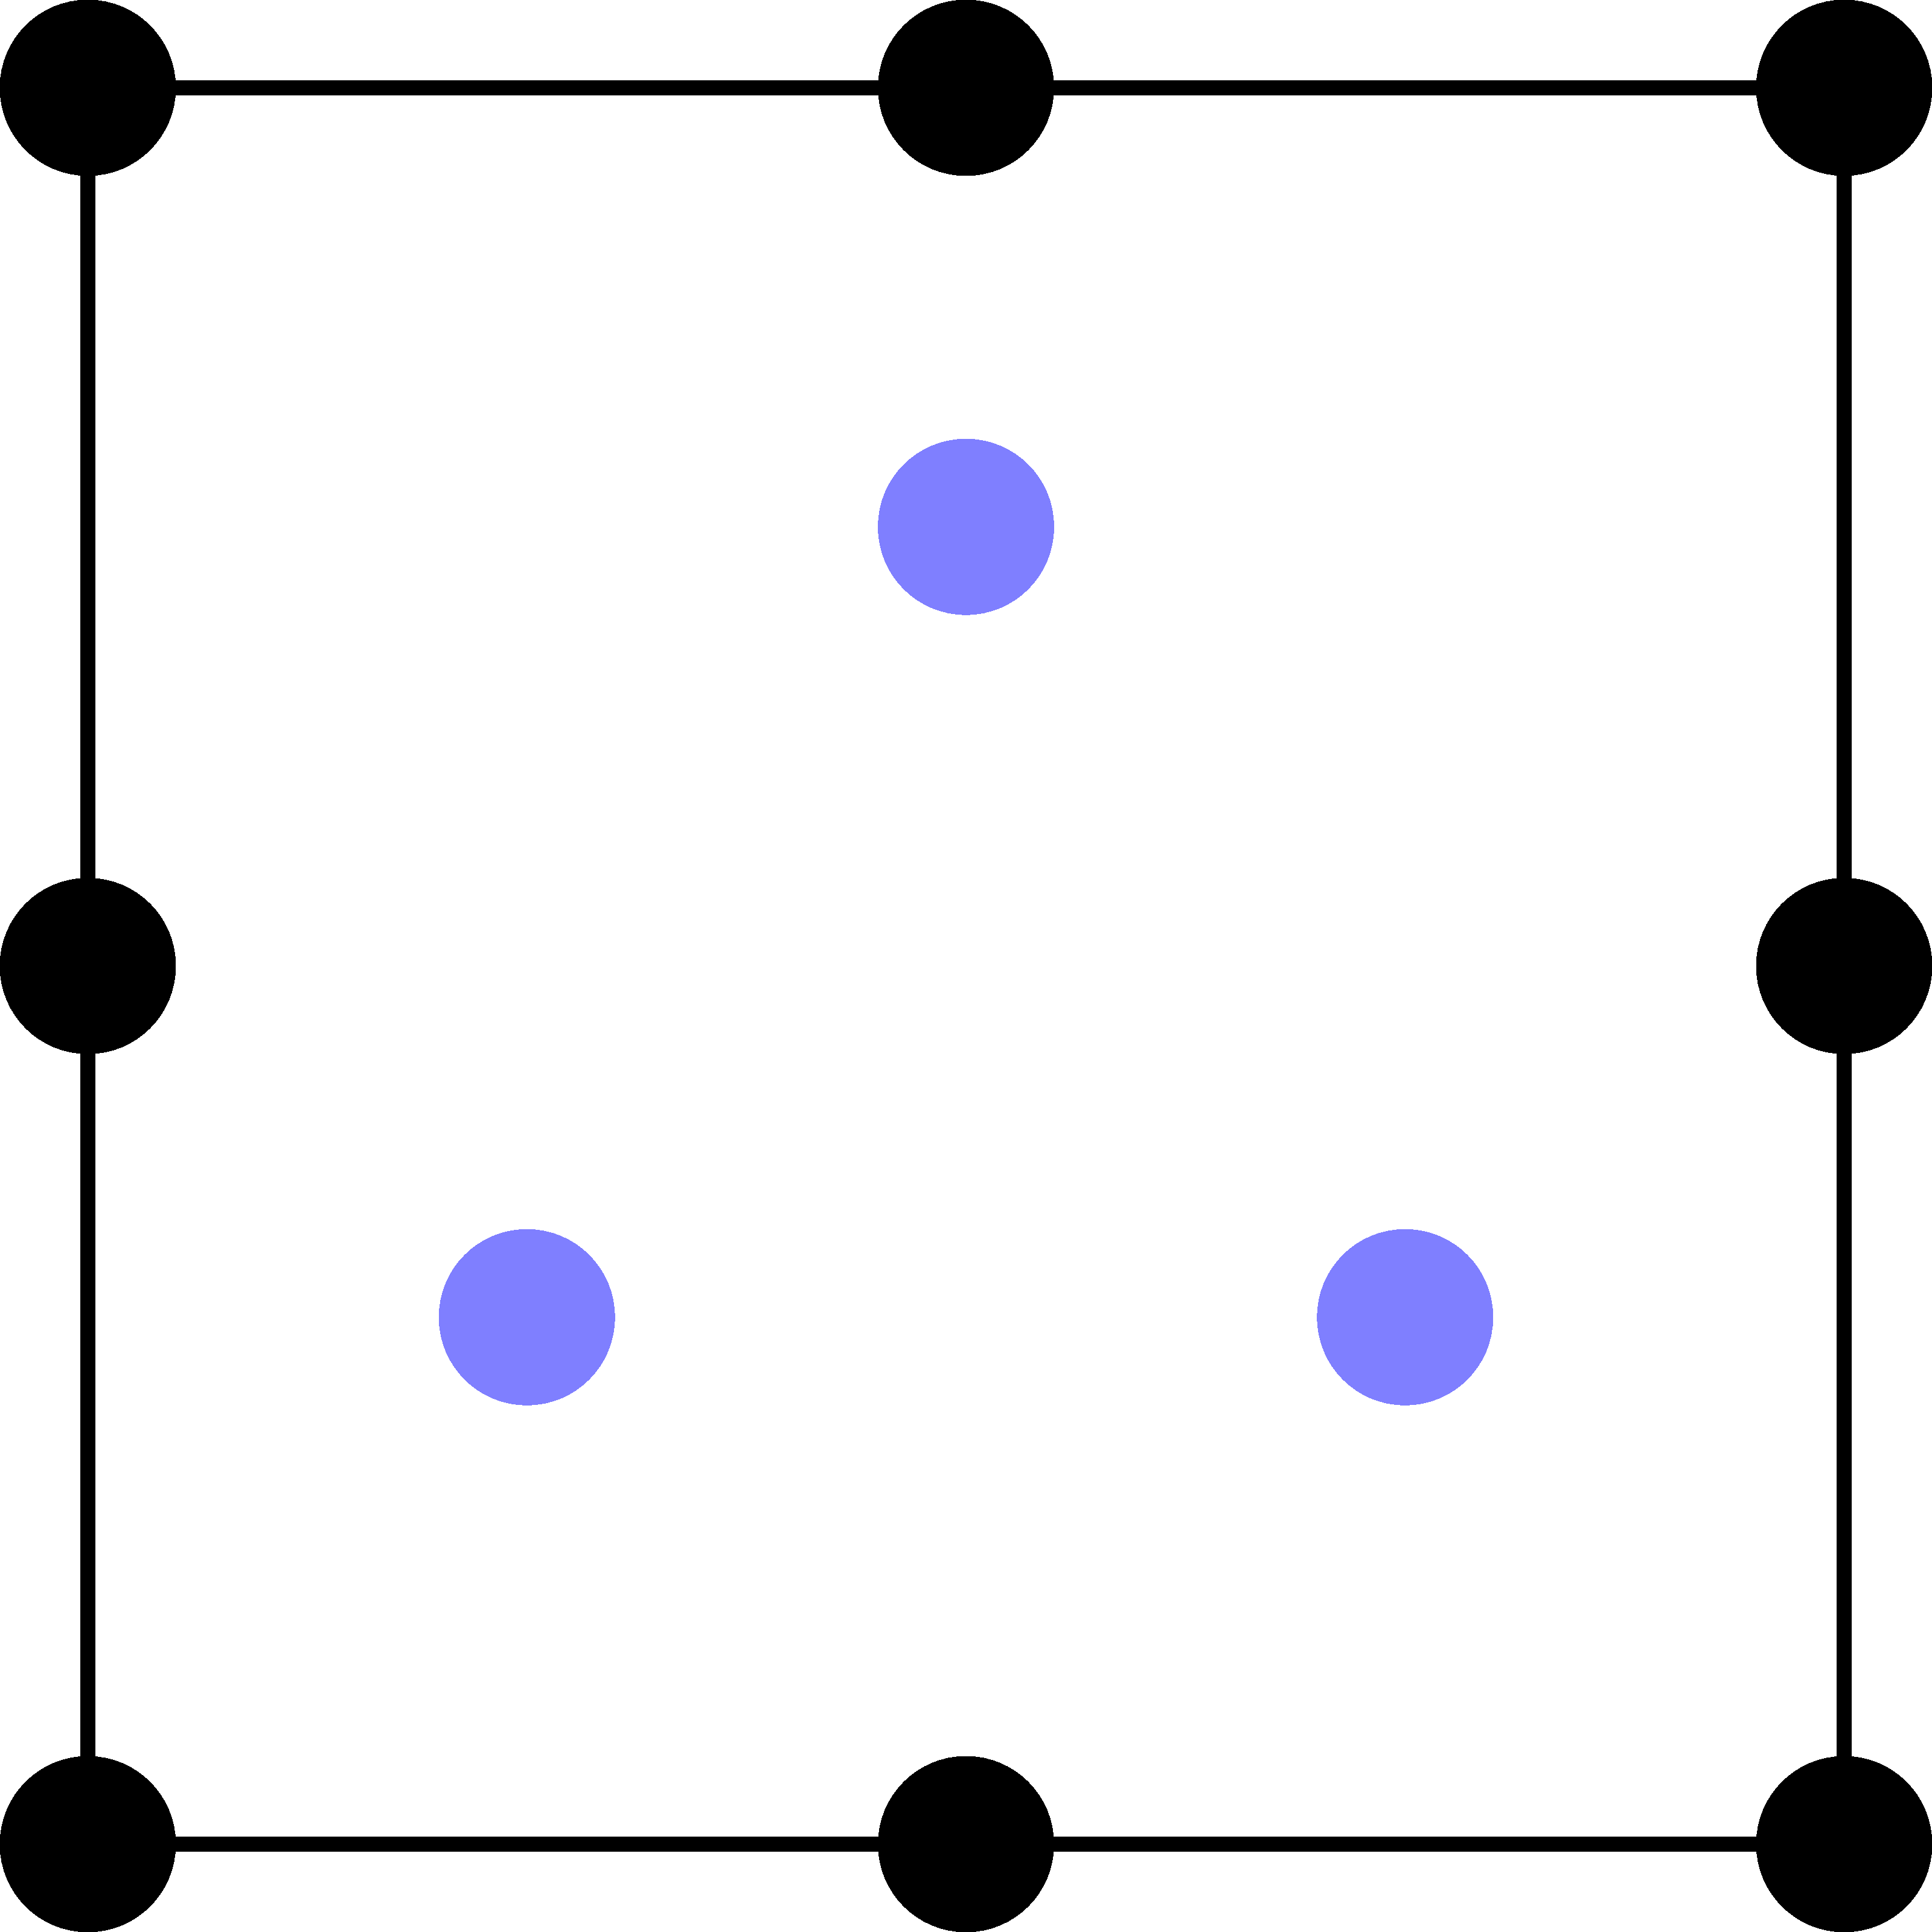
\includegraphics[width=0.9\textwidth]{figures/mix_Q8P3.png}
            \end{minipage}\\Q8P3
        \end{tabular}
        &2&$\times$ & $\times$\\
        \hline
        \begin{tabular}{c}
            \begin{minipage}{0.1\columnwidth}
                \centering
                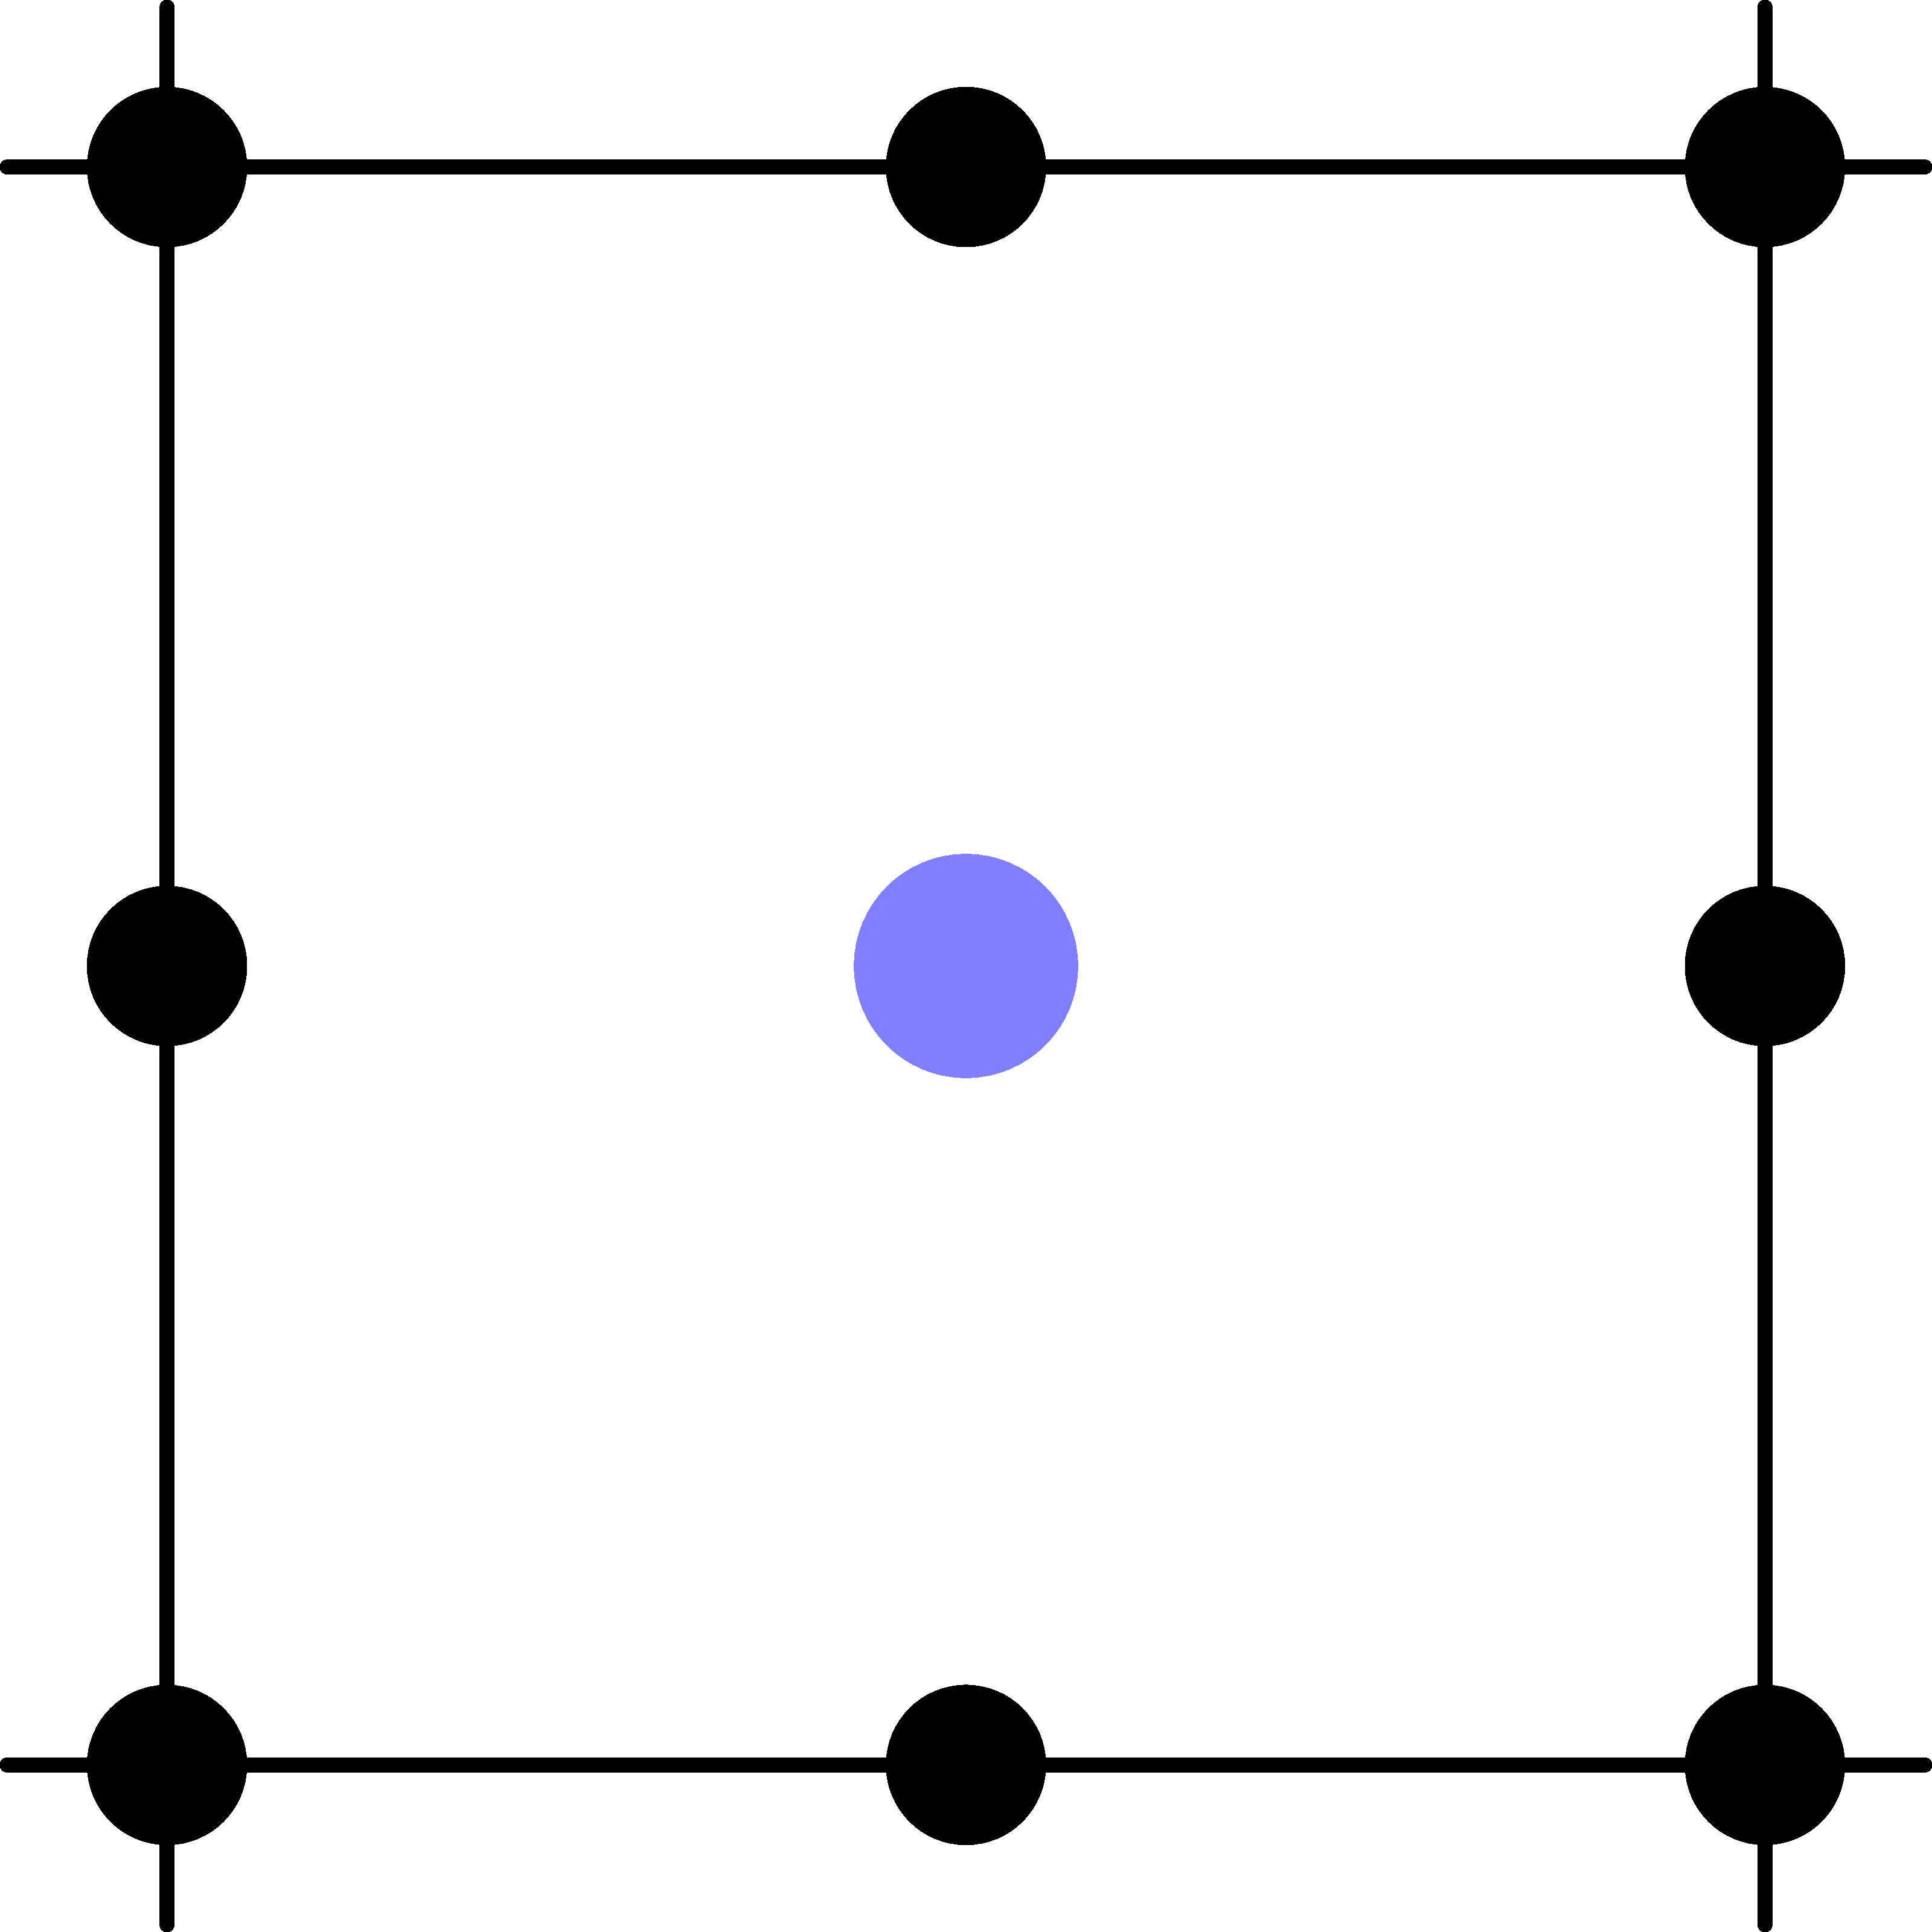
\includegraphics[width=0.9\textwidth]{figures/mix_Q8P1.png}
            \end{minipage}\\Q8P1
        \end{tabular}
        &6&\checkmark & \checkmark\\
        \hline
        \begin{tabular}{c}
            \begin{minipage}{0.1\columnwidth}
                \centering
                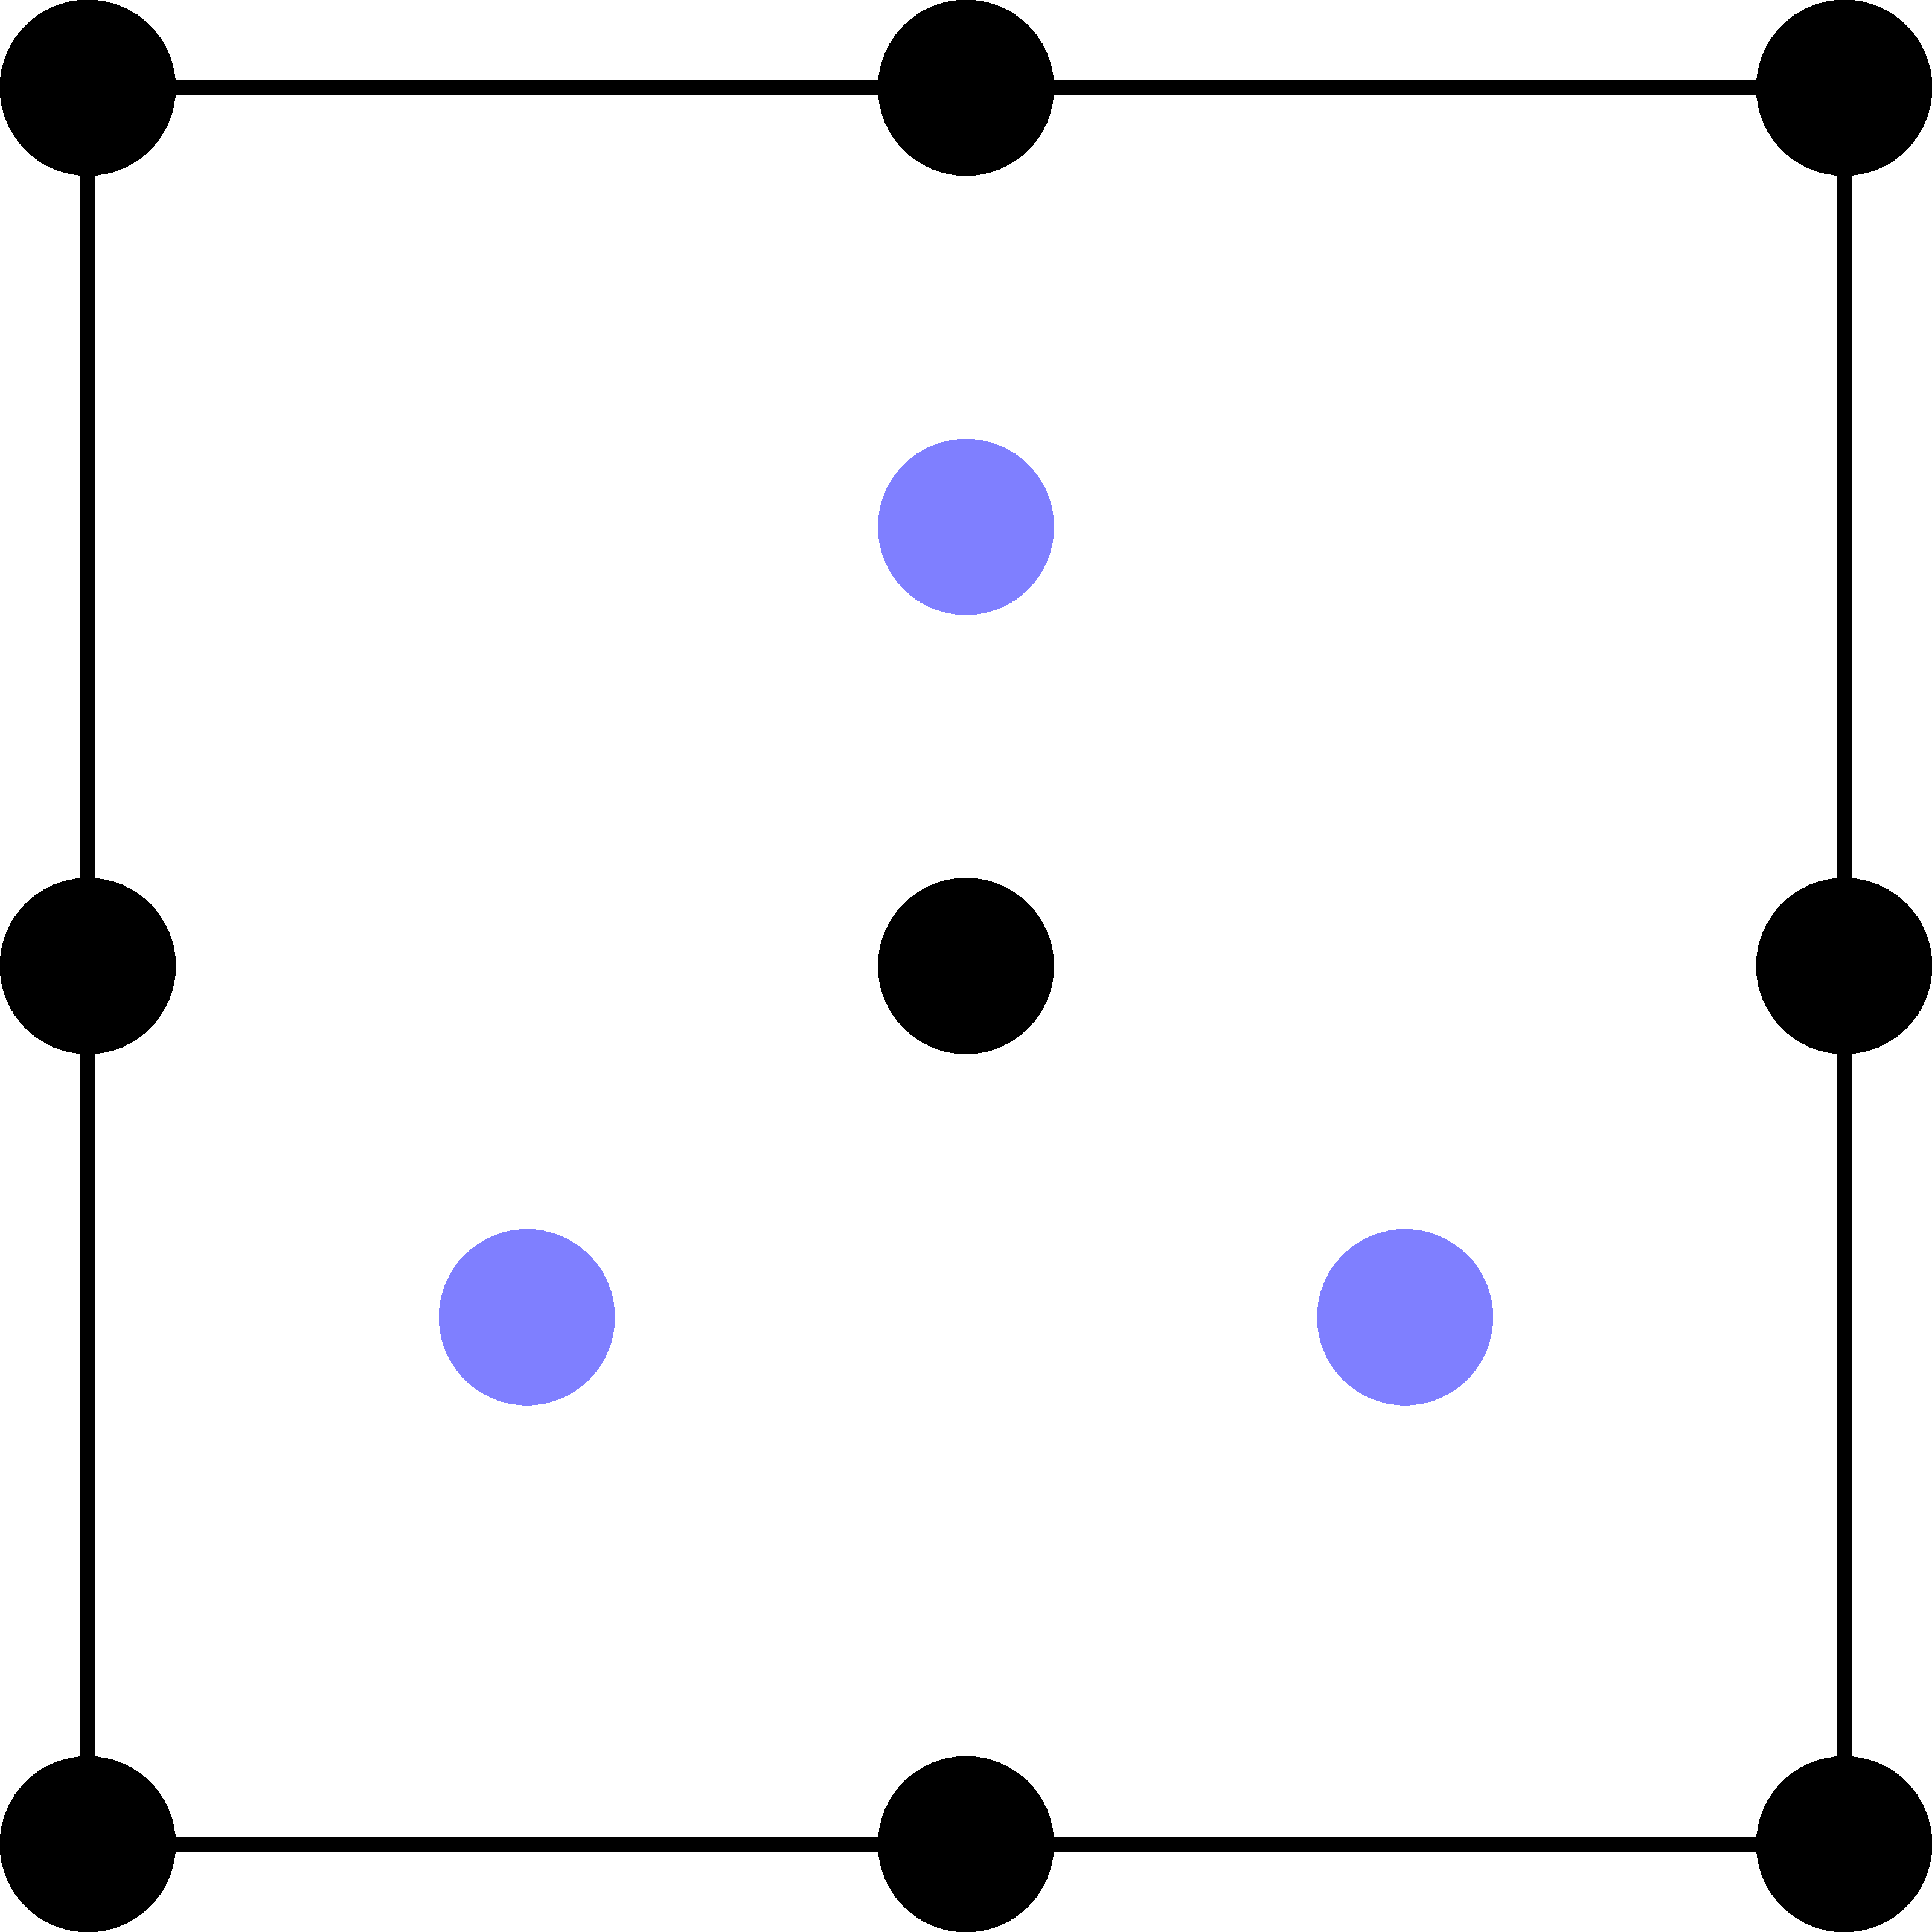
\includegraphics[width=0.9\textwidth]{figures/mix_Q9P3.png}
            \end{minipage}\\Q9P3
        \end{tabular}
        &$\frac{8}{3}$&\checkmark & \checkmark\\
        \hline
        \begin{tabular}{c}
            \begin{minipage}{0.1\columnwidth}
                \centering
                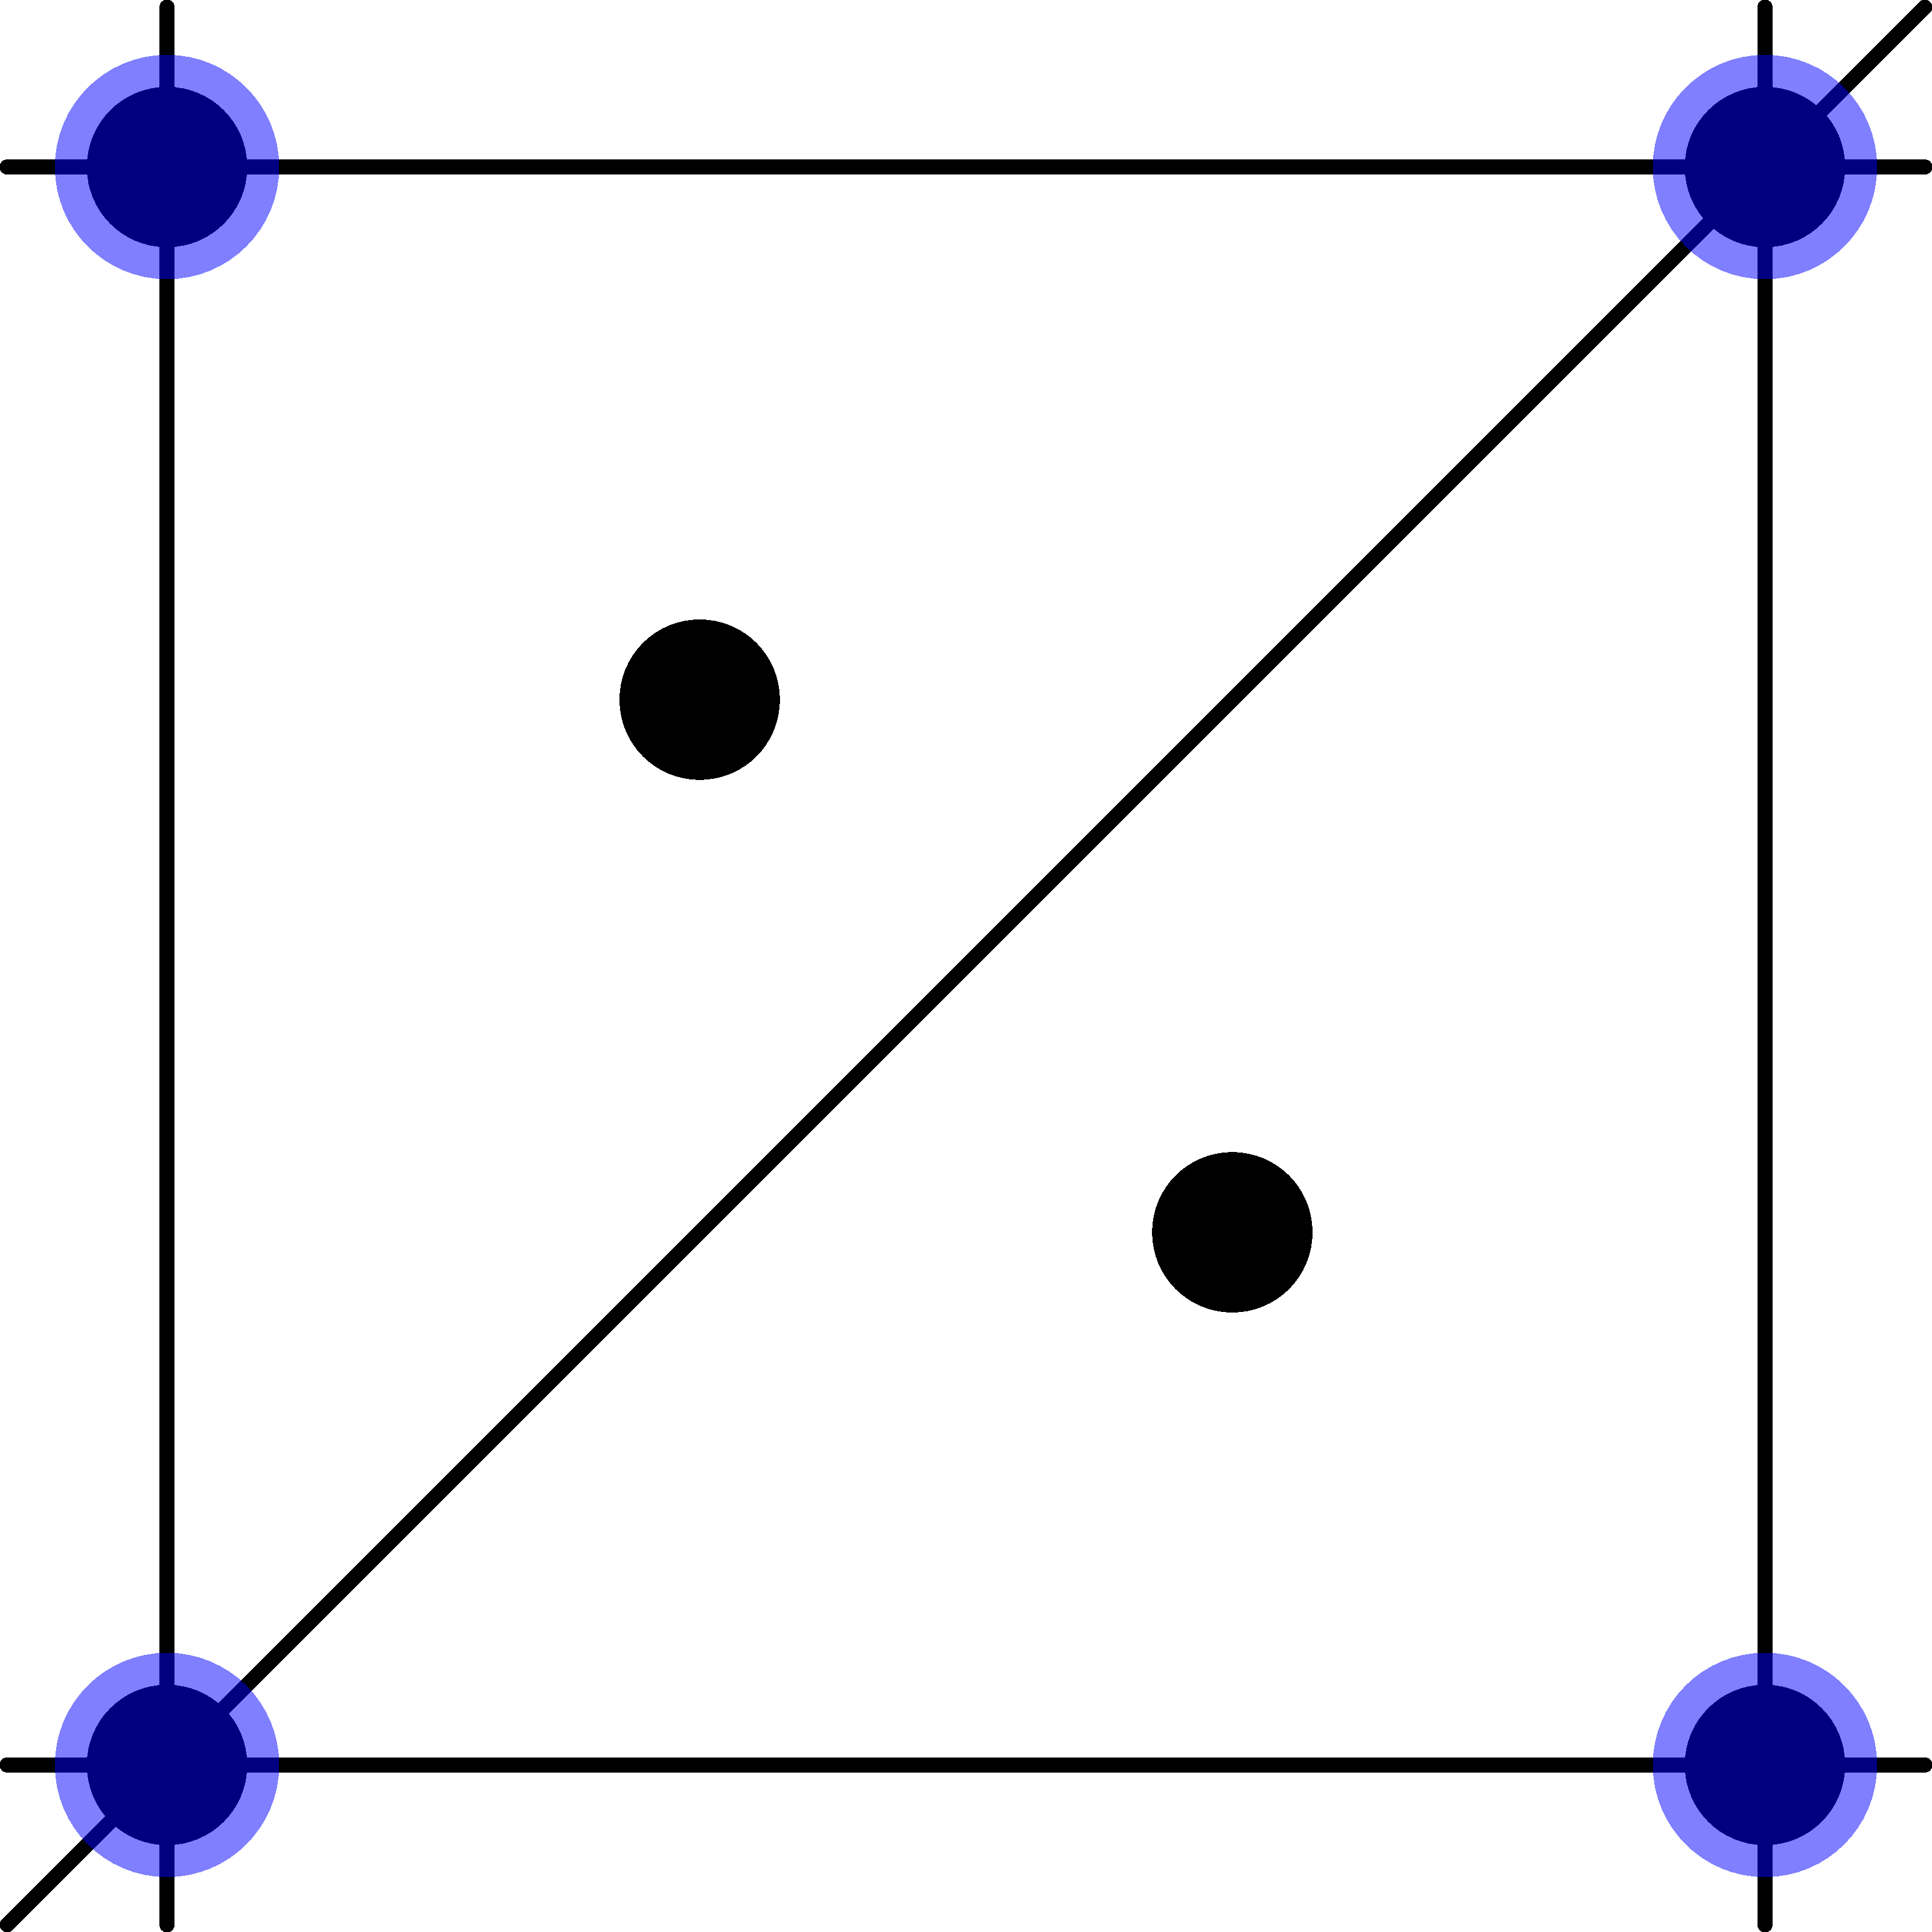
\includegraphics[width=0.9\textwidth]{figures/mini.png}
            \end{minipage}\\MINI element \cite{arnold1984,auricchio2005}
        \end{tabular}
        &$\frac{8}{3}$&\checkmark & \checkmark\\
        \hline
        \begin{tabular}{c}
            \begin{minipage}{0.1\columnwidth}
                \centering
                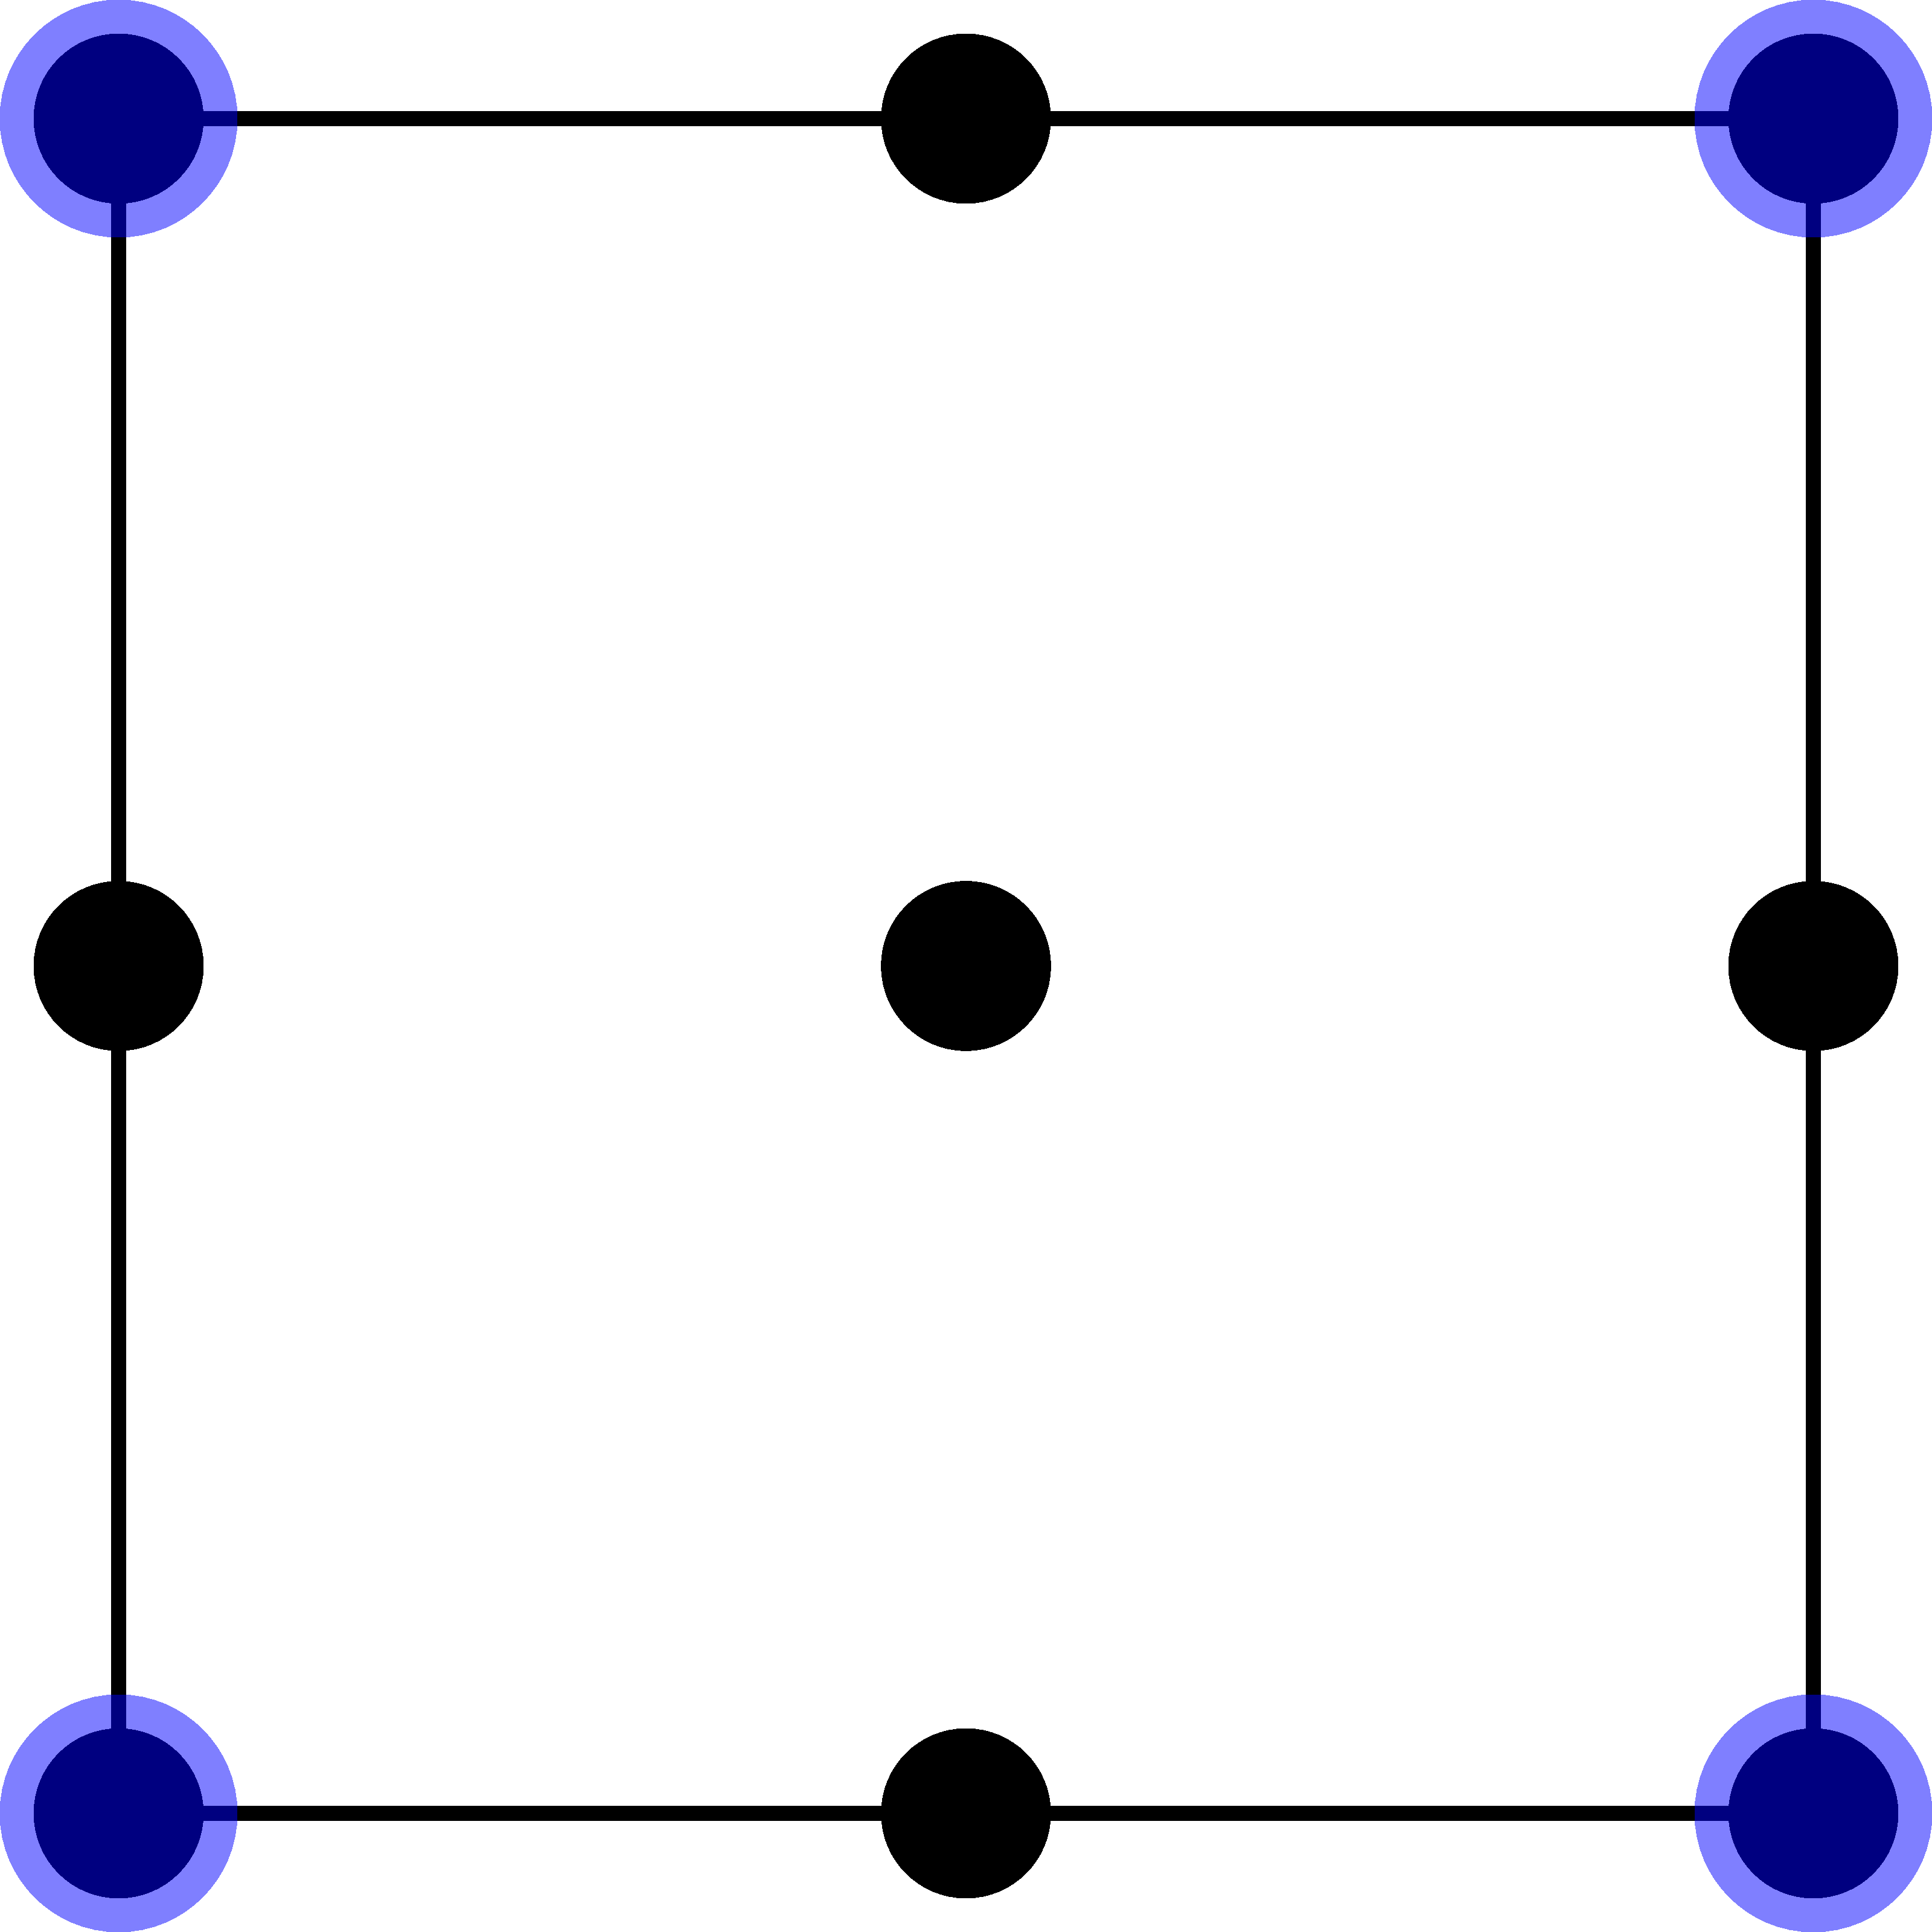
\includegraphics[width=0.9\textwidth]{figures/TaylorHood.png}
            \end{minipage}\\Taylor--Hood element \cite{hood1974}
        \end{tabular}c
        &$\frac{8}{3}$&\checkmark & \checkmark\\
        \hline
        \begin{tabular}{c}
            \begin{minipage}{0.1\columnwidth}
                \centering
                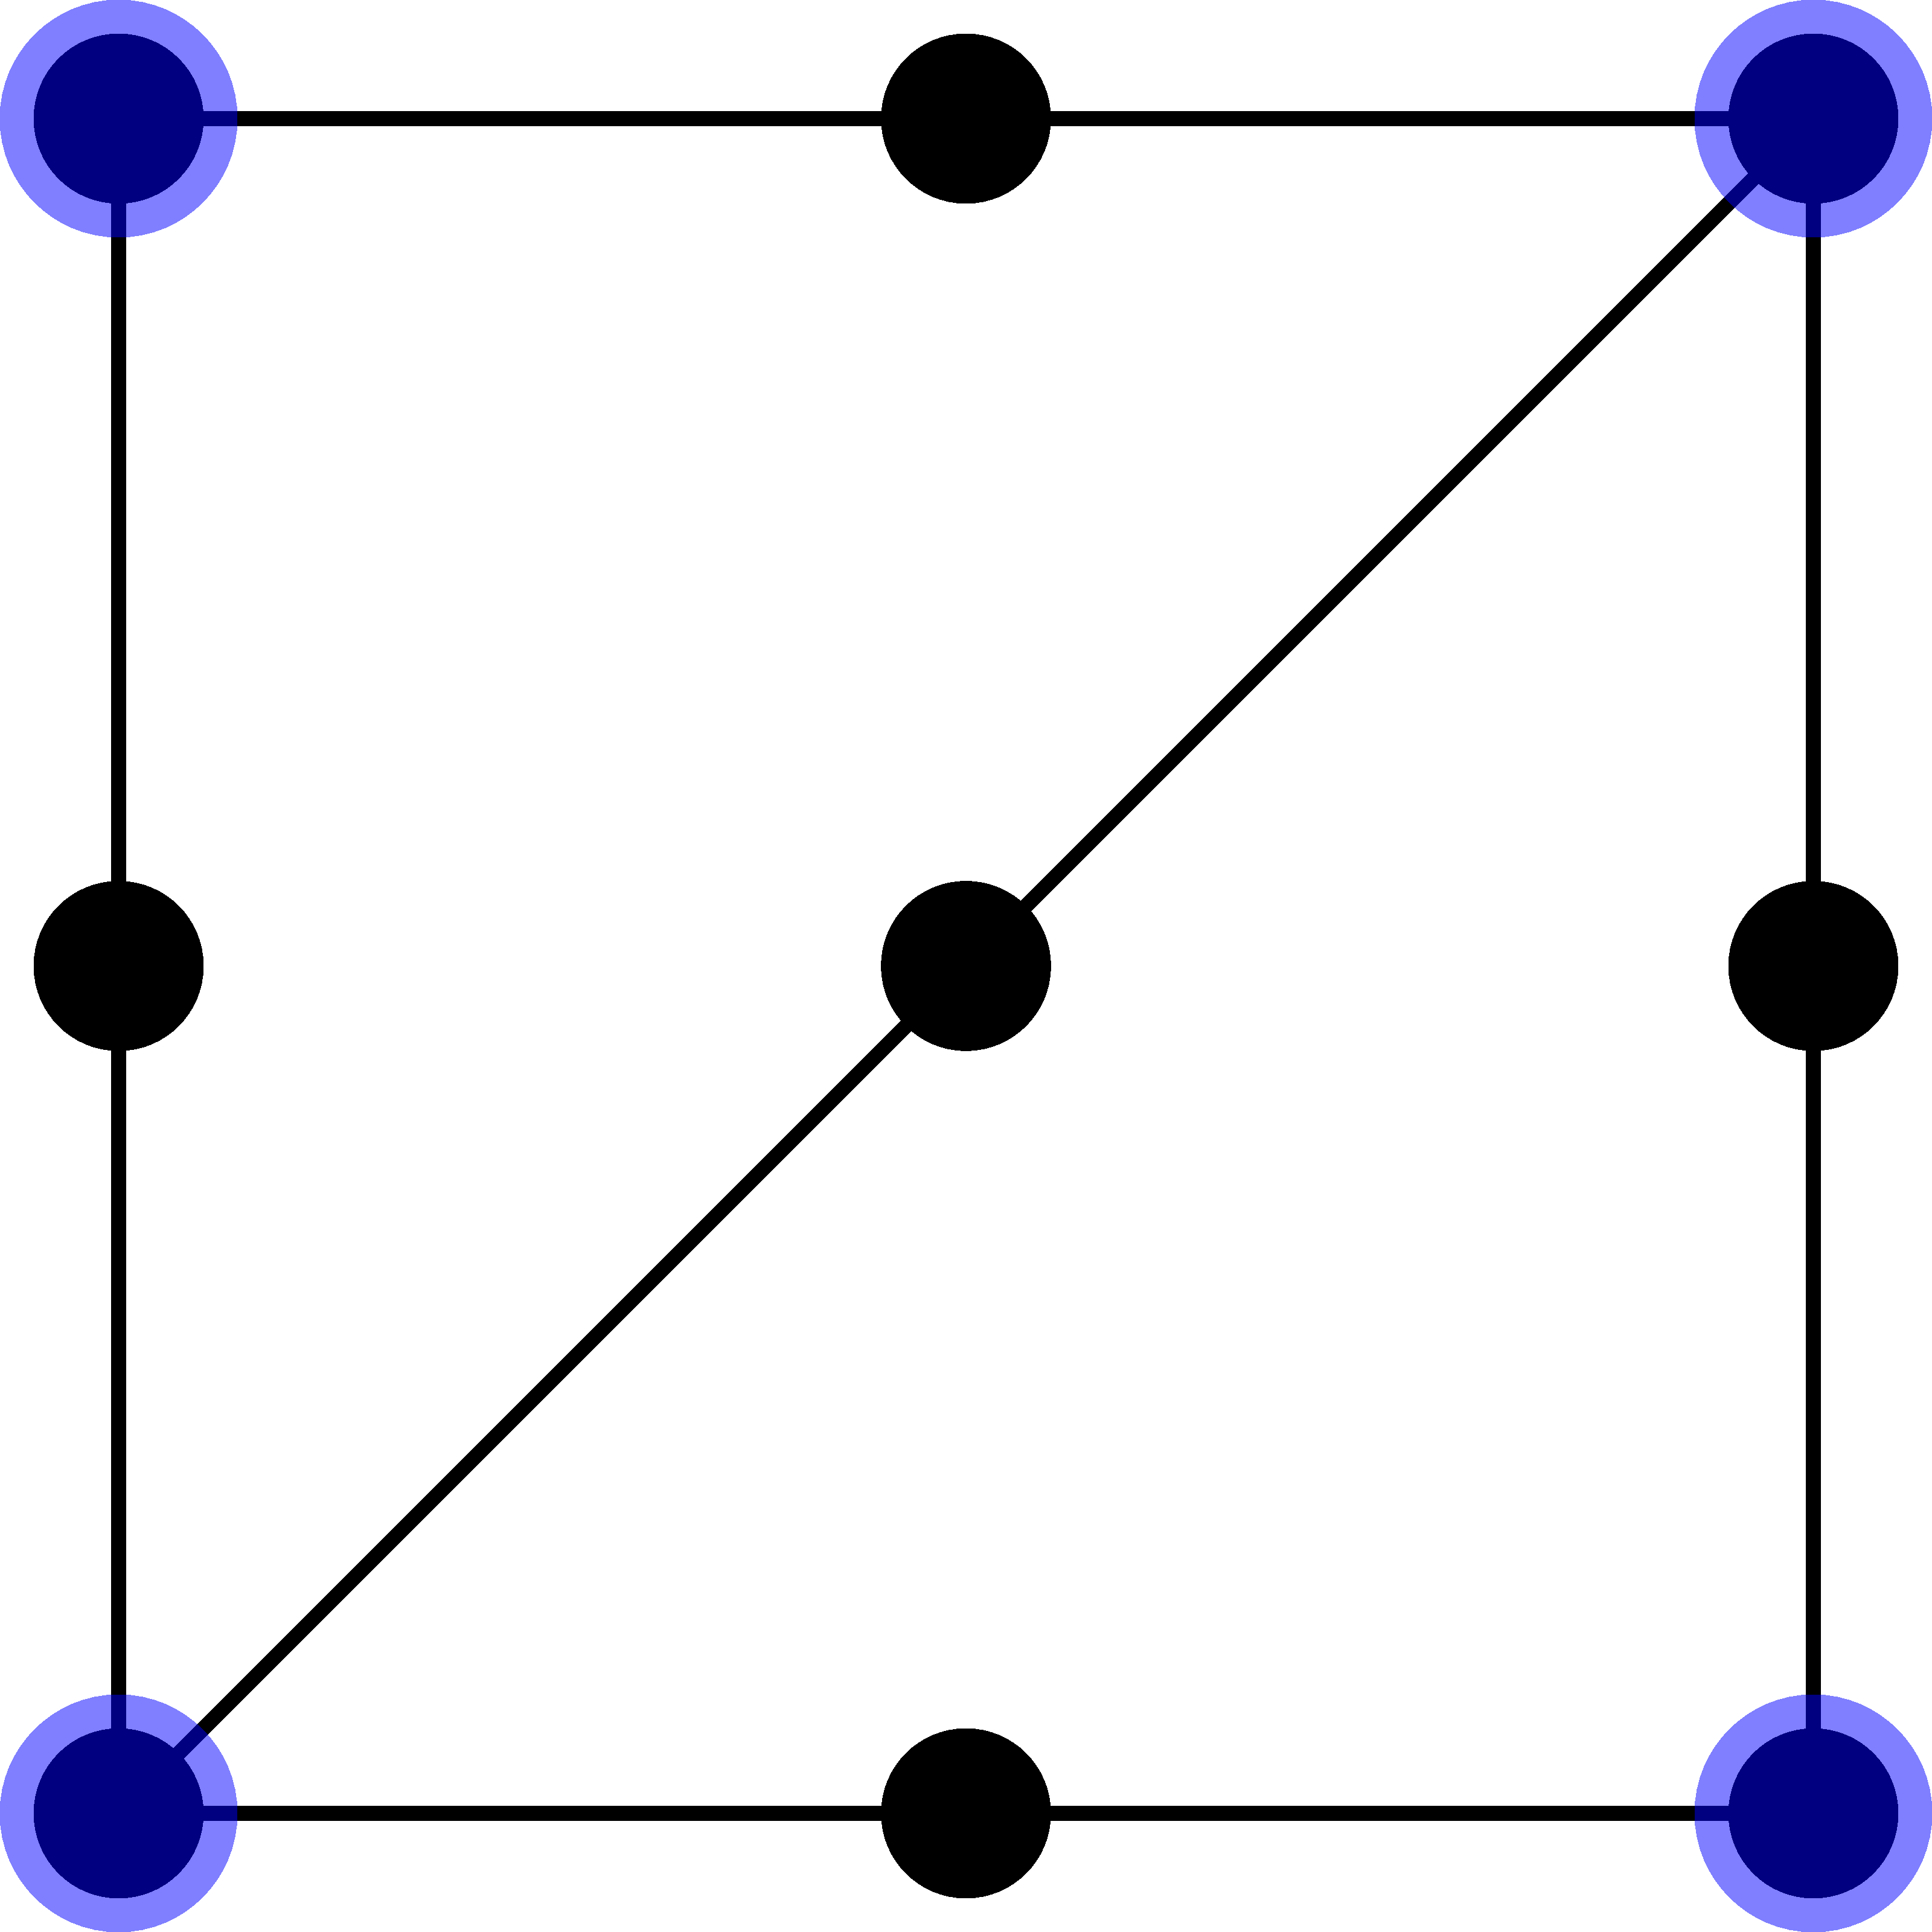
\includegraphics[width=0.9\textwidth]{figures/mix_T6C3.png}
            \end{minipage}\\T6C3
        \end{tabular}
        &8&\checkmark & \\
        \hline
        \begin{tabular}{c}
            \begin{minipage}{0.1\columnwidth}
                \centering
                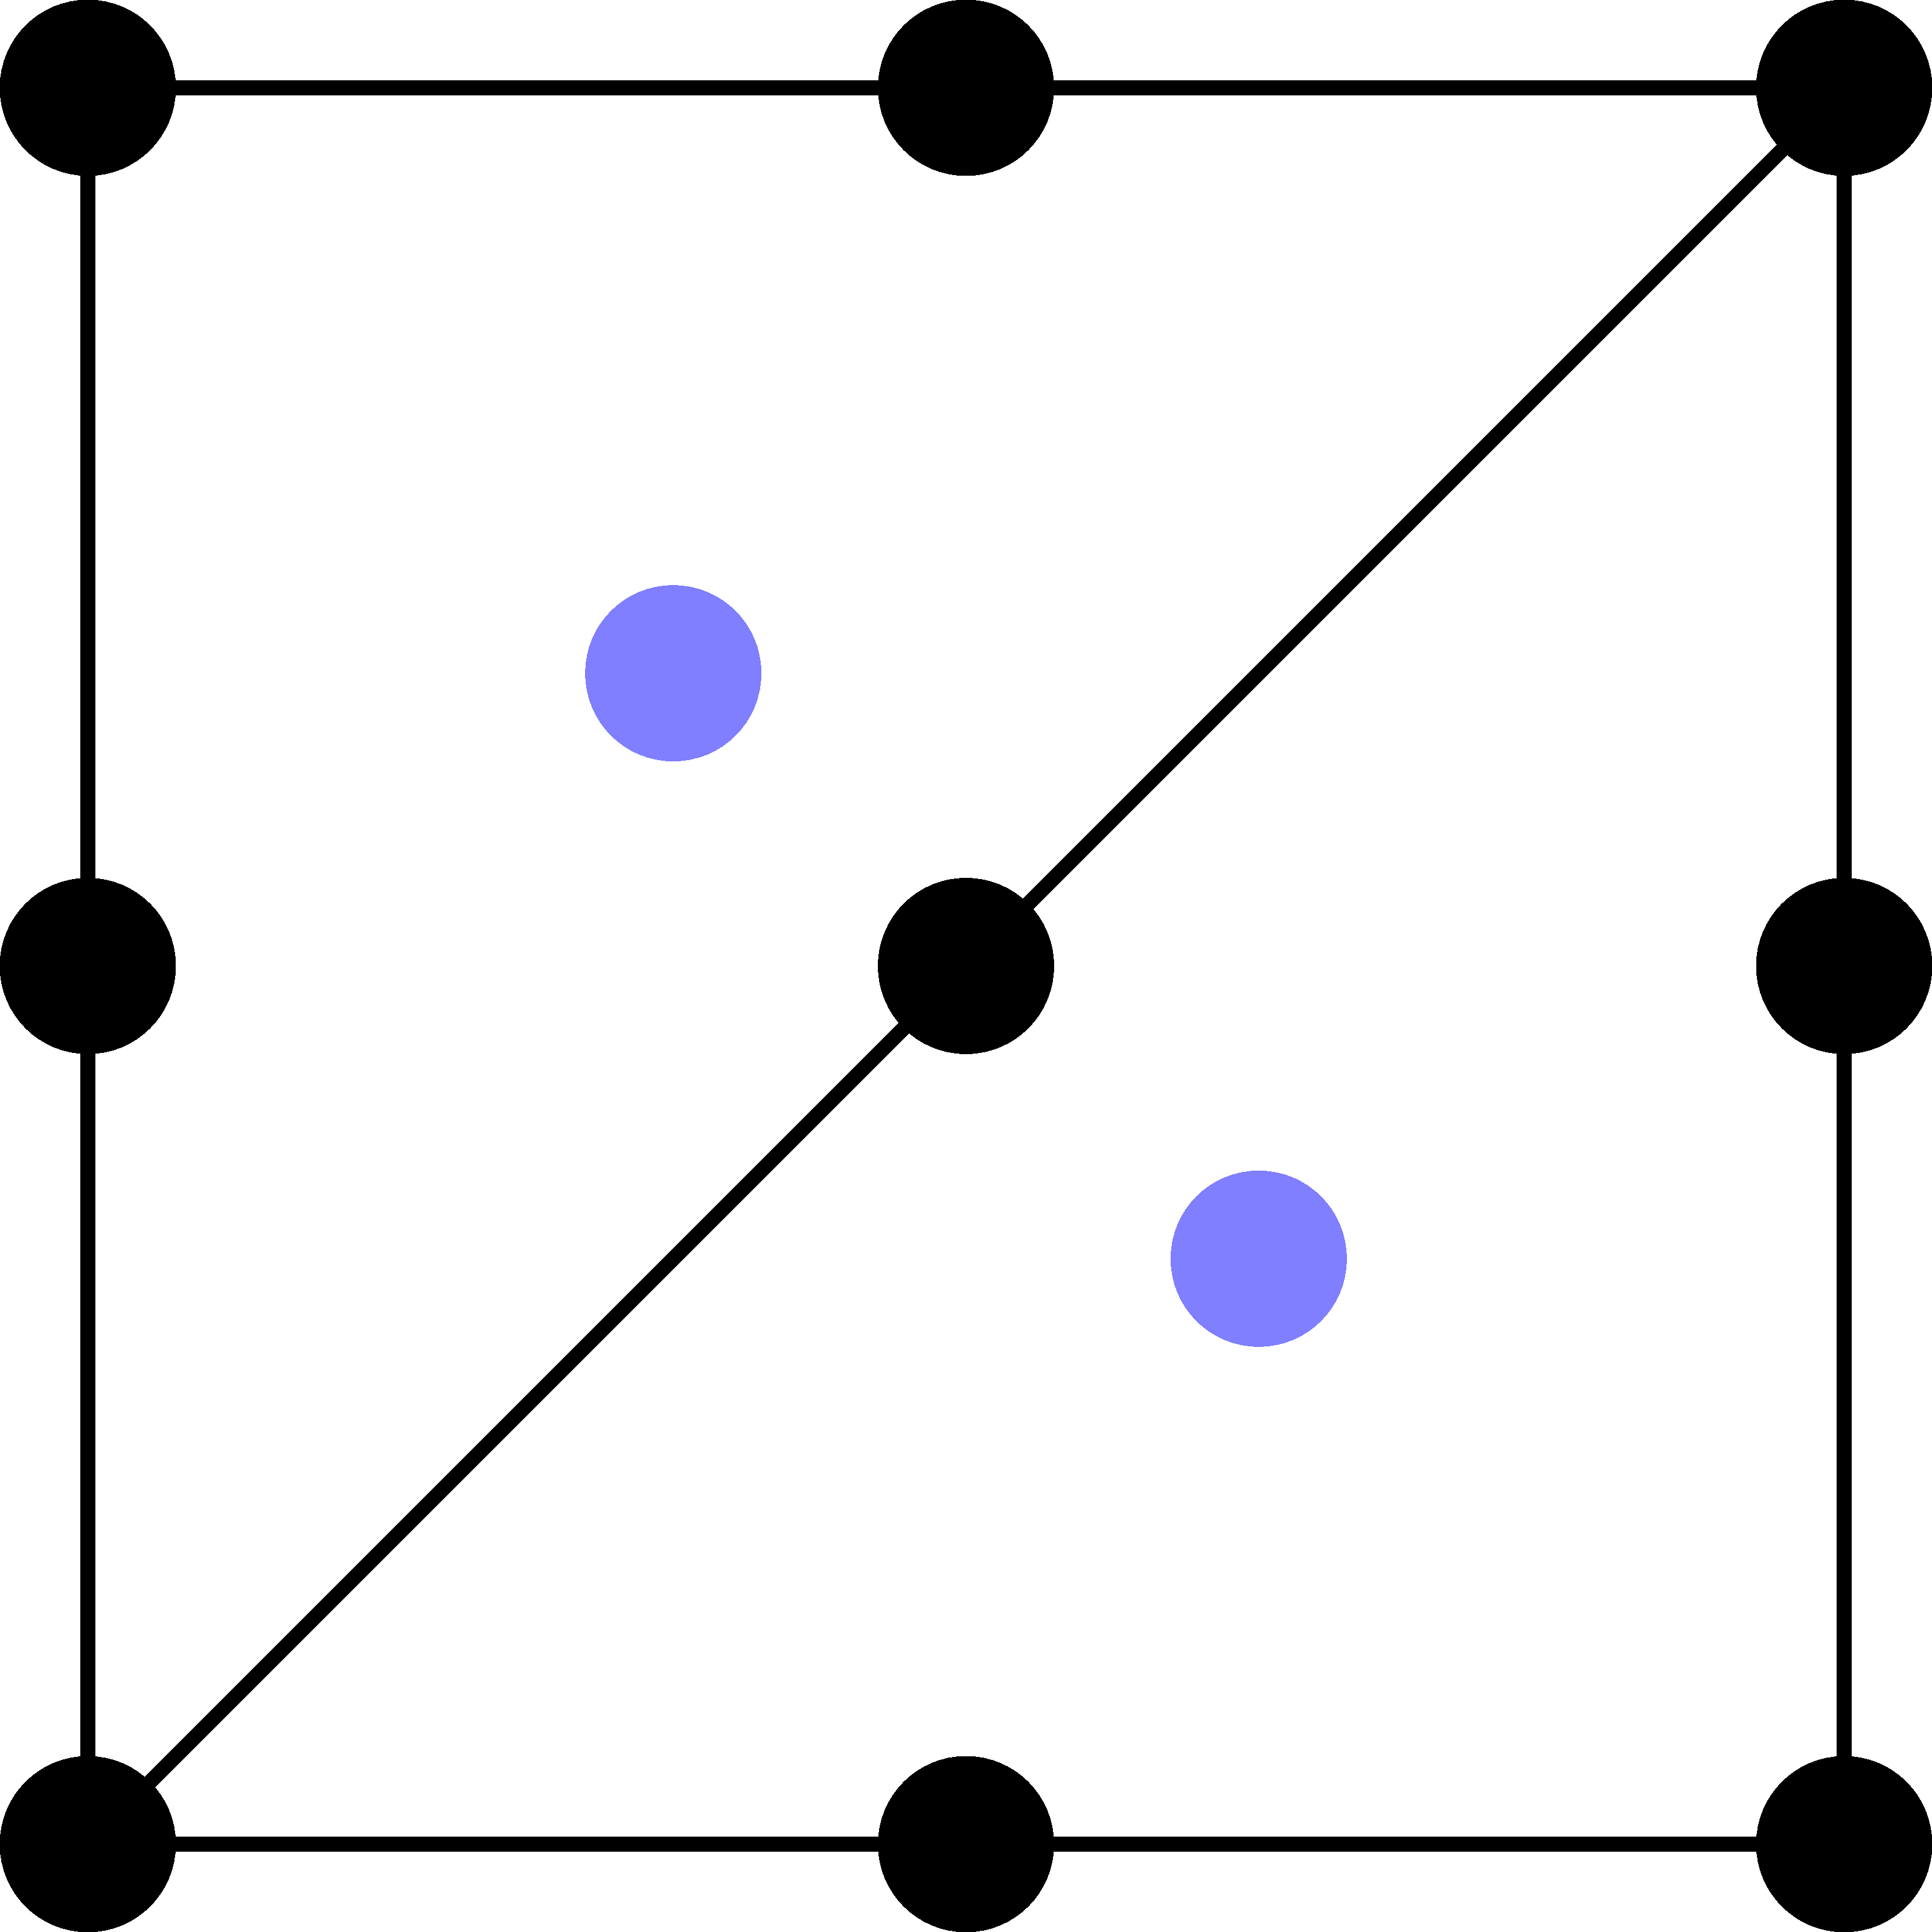
\includegraphics[width=0.9\textwidth]{figures/CrouzeixRaviart.png}
            \end{minipage}\\Crouzeix-Raviart element \cite{crouzeix1973}
        \end{tabular}
        &4&\checkmark & \\
        \hline
        \multicolumn{4}{c}{
                \begin{tabular}{c@{\hspace{24pt}}c}
                    \raisebox{-0.3\height}{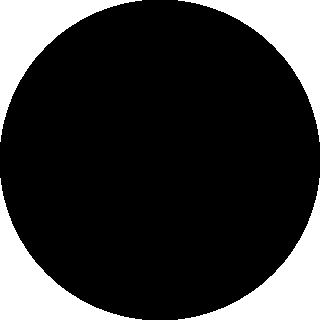
\includegraphics[width=14pt]{figures/legend_u.png}} :位移节点 &
                    \raisebox{-0.3\height}{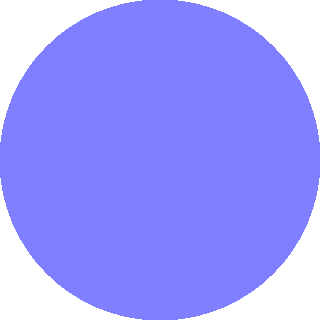
\includegraphics[width=14pt]{figures/legend_p.png}} :压力节点 
                \end{tabular}}\\
        \hline
    \end{tabular}
\end{table}
\section{小结}
本章讨论了体积自锁问题及其目前的解决方法。首先介绍了体积不可压材料的性质,随后详细讨论了通过罚函数法和拉格朗日乘子法两个常用的免体积自锁方法,且两种方法在数学上等价。
最后根据上述两种方法介绍了免体积自锁条件,包括体积约束比和LBB稳定性条件,并指出传统混合离散法无法同时满足最优约束比和LBB稳定性条件。
